\documentclass[11pt,oneside,openany]{book}
\usepackage{zlc_frontend_notes}

\begin{document}
\frontmatter
\zlctitlepage{Zou\_lab\_control.frontend 中文手册}{Jupyter / GUI 实验绘图前端}{统一 array 数据契约、live session、fit、selector 与 PDF notes}{2026-06-05}
\tableofcontents
\cleardoublepage
\mainmatter

\chapter{写给新读者}

\section{frontend 这一层做什么}
\pyapi{Zou_lab_control.frontend} 是独立的用户界面层，拥有：绘图、实时刷新、Fluent/PyQt 控件、脉冲编辑器、以及 PDF/手册渲染。它\tfocus{不}拥有任何硬件动作——脉冲编辑器只是 \pyapi{PulseTableState} 加一个传入 sequencer 的前端。

主要文件：

\begin{description}
  \item[\filepath{qt_fluent.py}] 可复用的 Fluent/Confocal 风格与控件，以及结构上防止裁切/重叠的布局原语。
  \item[\filepath{pulse_gui.py}] Confocal 风格脉冲编辑器，编辑 \pyapi{PulseTableState} 并调用传入的 \pyapi{SequencerDevice}。
  \item[\filepath{live.py}, \filepath{data_figure.py}, \filepath{canvas.py}] 绘图与实时刷新层。
  \item[\filepath{notes.py}] PDF/手册渲染（\pyapi{render_tex_pdf} 等）。
\end{description}

\begin{notebox}[一条总规则]
PyQt 前端应复用 \filepath{qt_fluent.py}，不要在每个 GUI 里手写一套 Qt 样式。布局应使用本章介绍的原语，而不是逐行硬编码像素几何——这是“对齐契约”能在不同 Windows DPI 下稳定成立的原因。
\end{notebox}

\chapter{qt\_fluent 控件库}

\section{视觉基调}
统一用 Segoe UI、12 pt、背景 \pyapi{#F3F3F3}、文字 \pyapi{#323130}、强调色 \pyapi{#77AADD}、圆角 4 px、柔和卡片阴影。\pyapi{FluentGroupBox} 是带灰色标题胶囊的白色卡片；保留无硬边框、软阴影的样式，不要为了“更显眼”加硬轮廓，也不要把编辑器换成普通表格。用 \pyapi{FluentComboBox}/\pyapi{FluentSpinBox}/\pyapi{FluentScrollArea} 让弹出列表、计数器、细滚动条共享同一套样式。

\section{缩放：一套，不是两套}
所有固定几何用 \pyapi{set_fluent_scale()} / \pyapi{scaled_px()}。不要在某个 GUI 模块里再造第二套缩放系统。

\section{布局原语（结构上防裁切/重叠）}
下面这些是新加入的原语。优先用它们，而不是逐行 \pyapi{setFixedGeometry}：

\begin{description}
  \item[\pyapi{Metrics}] 缩放后的间距/尺寸 token：\pyapi{margin/gap_row/gap_item/gap_tight/row_h/dot}。在使用时再读取，它们随当前 DPI 缩放变化。
  \item[\pyapi{measure_text_width(texts, ...)}] 按当前缩放返回能容下最宽文本的标签列宽。让标签列宽“由内容驱动”，避免写死宽度导致 \pyapi{cooling_pgc}、\pyapi{da_dipole} 这类名字被截断。
  \item[\pyapi{ElidedLabel}] 文本过长时用 \pyapi{...} 省略，并把完整文本放进 tooltip。
  \item[\pyapi{FluentScanDot}] 字段旁的圆形开关：未绑定时是空心灰点；绑定后是实心橙点，中间显示它的 1-based slot 编号。
  \item[\pyapi{mark_scan_field(widget, bound=...)}] 给绑定到 slot 的字段套上“橙色 + 禁用”外观。
  \item[\pyapi{FluentLabeledField} / \pyapi{FluentFormGrid}] \pyapi{label : widget} 行，标签列共享、对齐，每行同高。把一摞表单堆叠起来时天然对齐，不需要逐行写死几何。
\end{description}

\begin{figure}[htbp]
  \centering
  \begin{tikzpicture}[font=\footnotesize]
    \node[draw=StarkPale, rounded corners=2pt, minimum width=22mm, minimum height=7mm, anchor=west] (lab) at (0,0) {Step:};
    \node[draw=StarkPale, rounded corners=2pt, fill=StarkCodeBack, minimum width=30mm, minimum height=7mm, anchor=west] (edit) at (2.4,0) {20 ns};
    \filldraw[StarkGray] (5.8,0) circle (2.2mm);
    \node[white, font=\bfseries\scriptsize] at (5.8,0) {1};
    \node[anchor=west, font=\scriptsize, text width=42mm] at (6.4,0) {一行 FluentLabeledField：对齐的标签列 + 字段 + 可选的 FluentScanDot（这里已绑定为 slot 1）。};
  \end{tikzpicture}
  \caption{标签列对齐 + 扫描圆点的一行表单。绑定后字段变橙并禁用。}
  \label{fig:fe-field}
\end{figure}

\section{用原语搭一个对齐的页面}
一个稳健、对齐的 Fluent 页面的骨架：

\begin{codeblock}[Python]
from Zou_lab_control.frontend import qt_fluent as qf

label_w = qf.measure_text_width(["Step:", "Use Y:", "Scan XY:"])  # 由内容决定列宽
form = qf.FluentFormGrid(label_width=label_w)
form.add_row("Step:", qf.FluentLineEdit("20"))
form.add_row("Total:", qf.FluentLineEdit("1.2 ms"))
# 每行同高 (Metrics.row_h())，标签列共享 label_w；堆叠时自动对齐。
\end{codeblock}

\chapter{脉冲编辑器}

\section{三个标签页}
\pyapi{PulseSequenceEditor} 有 \tfocus{Edit / Preview / Scan} 三个标签页。

\begin{figure}[htbp]
  \centering
  \begin{tikzpicture}[font=\footnotesize,
      tab/.style={draw=StarkTeal, fill=StarkTint, rounded corners=2pt, minimum width=22mm, minimum height=8mm},
      panel/.style={draw=StarkPale, fill=StarkCodeBack, rounded corners=2pt, align=center, font=\scriptsize, inner sep=3pt}]
    \node[tab] (e) {Edit};
    \node[tab, right=2mm of e] (p) {Preview};
    \node[tab, right=2mm of p] (s) {Scan};
    \node[panel, below=3mm of e, text width=30mm, minimum height=20mm, anchor=north west] (ep)
      {Channel Names\\Delay \& Scan\\period 卡片时间线\\Control Buttons\\Channel View};
    \node[panel, below=3mm of p, text width=30mm, minimum height=20mm, anchor=north west] (pp)
      {plot(kind="pulse")\\未展开周期表\\repeat 用 $\times\infty$ / $\times N$\\Show off rows 开关};
    \node[panel, below=3mm of s, text width=30mm, minimum height=20mm, anchor=north west] (sp)
      {写 Python 构造\\scan\_table\\(N\_points x N\_slots)\\Run};
  \end{tikzpicture}
  \caption{编辑器三页：Edit 编脉冲表，Preview 画未展开的时序图，Scan 写代码生成扫描表。}
  \label{fig:fe-tabs}
\end{figure}

\section{Edit 页}

\begin{figure}[htbp]
  \centering
  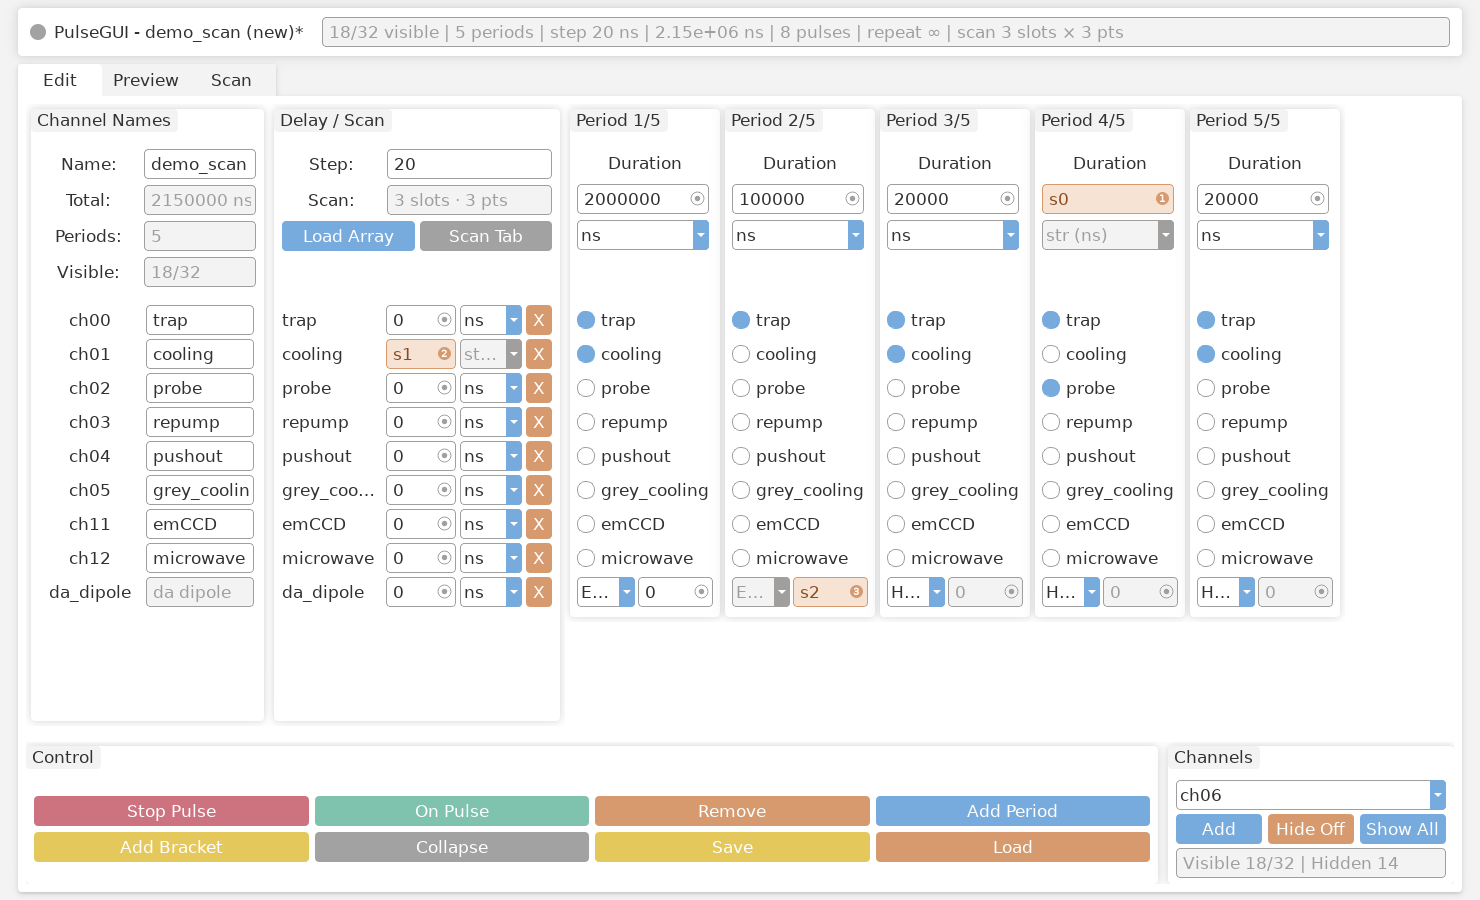
\includegraphics[width=\textwidth]{assets/frontend_gui_edit.png}
  \caption{Edit 标签页的真实截图（脱机离屏渲染）。左侧 Channel Names 与 Delay / Scan 列，中间是横向滚动的 period 卡片时间线，下方是 Control / Channels 控制条。橙色字段是已绑定到扫描 slot 的字段，字段右侧的圆点显示它的 slot 编号。}
  \label{fig:fe-edit-shot}
\end{figure}

按区域理解：

\begin{description}
  \item[\pyapi{Channel Names and Duration}] 脉冲名、总时长、period 数、可见数。左侧 raw 列在能读到 XDC 时显示物理 package pin（如 \pyapi{M17/M13}）；\pyapi{chNN} 保存在 tooltip 和 JSON/API state。右侧是可选的显示标签。
  \item[\pyapi{Delay \& Scan}] \pyapi{Step}（来自当前 sequencer 时钟，默认 20 ns）、每条可见 channel 的延时、以及 \pyapi{Load}（载入扫描表文件）和 \pyapi{Scan Tab}（打开 Scan 页）。
  \item[period 卡片时间线] 每张卡是一段持续时间，不是网格表。卡片含 duration、单位选择、位置（\pyapi{Period 1/5}）和每条 channel 的勾选框。
  \item[\pyapi{Control Buttons}] \pyapi{On Pulse}/\pyapi{Stop Pulse}、增删 period、repeat bracket、保存/读取。\pyapi{On Pulse} 先 prepare/上传当前脉冲再 start；GUI 没有独立 sync 按钮。
  \item[\pyapi{Channel View}] 从隐藏列表加回 channel、隐藏全程 off 的 channel、显示全部。
\end{description}

\begin{notebox}[对齐契约]
channel 名列、延时列、period 勾选框列共享\tfocus{同一个}竖直滚动位置。period 卡片可以横向滚动（当作时间线），但它们\tfocus{不能}有各自独立的竖直滚动条。同一条 channel 的 raw 标签、延时框、第一个 period 勾选框，三者的 \pyapi{mapTo(editor, QPoint(0,0)).y()} 必须相等。
\end{notebox}

\section{按字段扫描点工作流}

\begin{figure}[htbp]
  \centering
  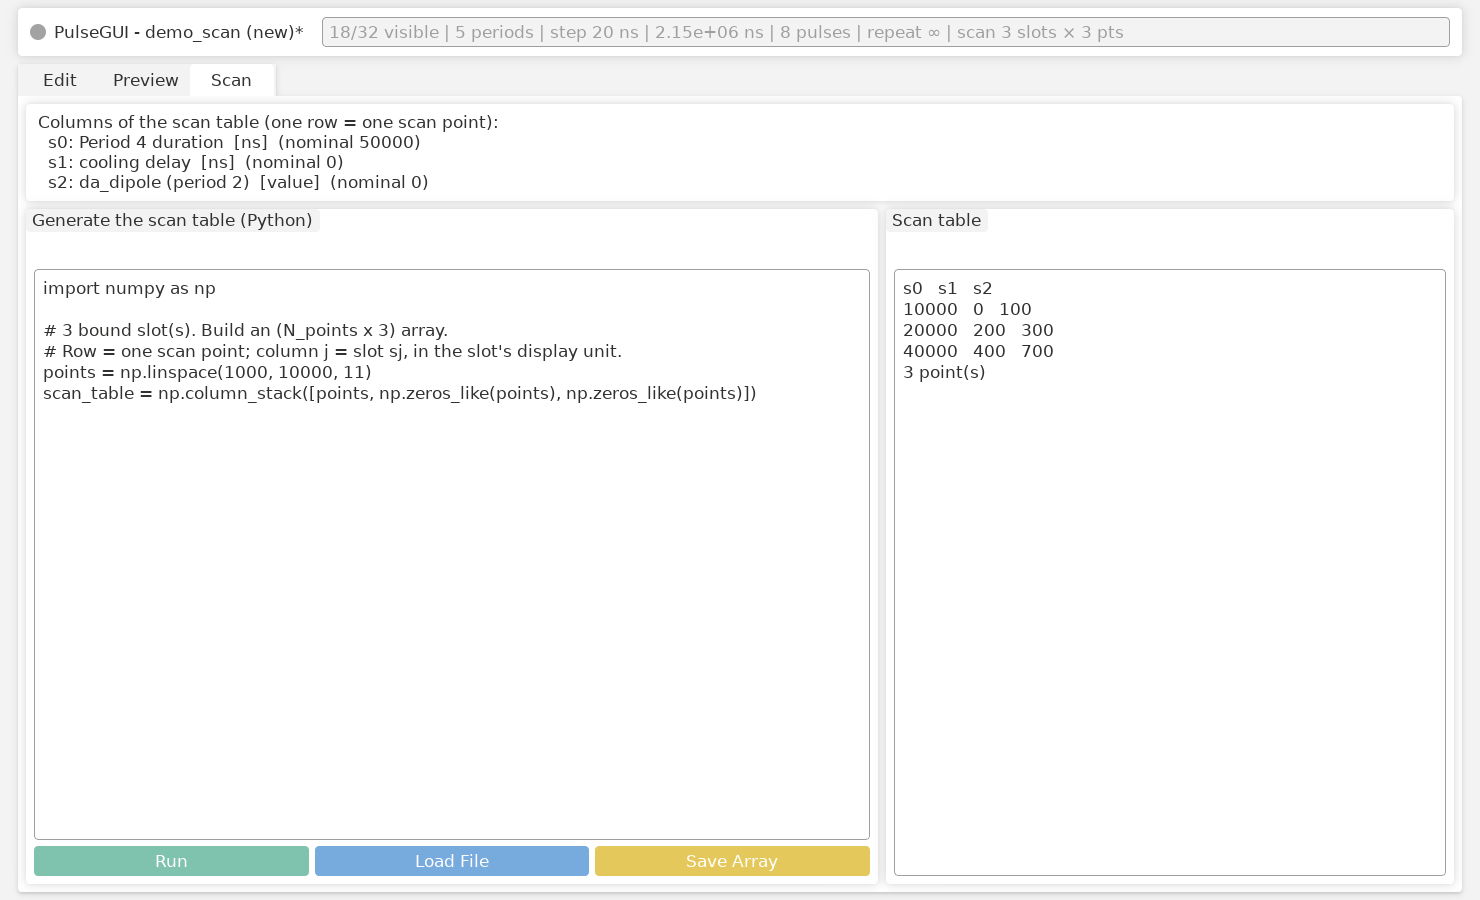
\includegraphics[width=\textwidth]{assets/frontend_gui_scan.png}
  \caption{Scan 标签页的真实截图。顶部列出扫描表的各列（每个绑定的 slot 一列，含它绑的字段与单位）；中间是 Python 代码框，运行后把 \pyapi{scan_table} 写回 state；底部是扫描表预览与 Run / Load File / Save Array 按钮。}
  \label{fig:fe-scan-shot}
\end{figure}

扫描以\tfocus{命名 slot}为单位（\pyapi{s0, s1, ...}），没有 x/y。

\begin{enumerate}
  \item 在 Edit 页点某个 duration / delay / DAC 字段旁的\tfocus{扫描圆点}。该字段变橙、禁用，并显示它的 slot 编号；这等价于 API 的 \pyapi{state.bind_field(kind, target)}。
  \item 打开 \tfocus{Scan} 页，写 Python 把一个 \pyapi{N_points x N_slots} 数组赋给变量 \pyapi{scan_table}。命名空间里有 \pyapi{np}、\pyapi{math}、\pyapi{n_slots}。
  \item 点 \pyapi{Run}，把表写回 state；或用 \pyapi{Load} 直接从 \filepath{.npy}/\filepath{.csv}/\filepath{.txt} 载入。
\end{enumerate}

\begin{codeblock}[Scan 页里的代码]
import numpy as np
# n_slots 个已绑定 slot。行 = 一个扫描点，列 j = slot sj（该 slot 的显示单位）。
points = np.linspace(1000, 10000, 11)
scan_table = points.reshape(-1, 1)        # 单 slot 时
# 多 slot 时，例如两列:
# scan_table = np.column_stack([points, points / 2])
\end{codeblock}

\section{Preview 页}

\begin{figure}[htbp]
  \centering
  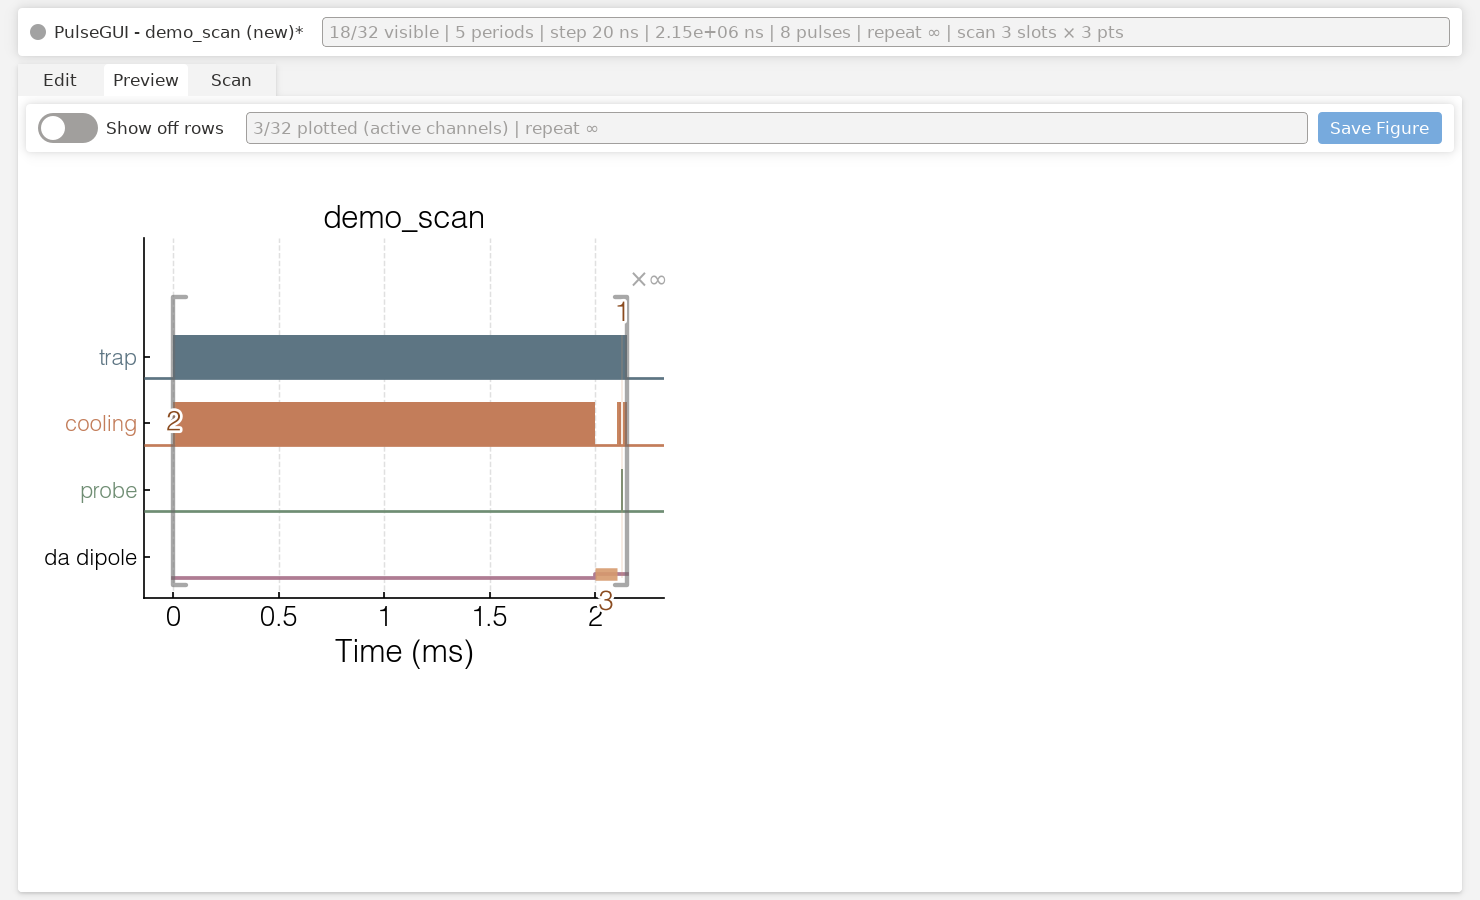
\includegraphics[width=\textwidth]{assets/frontend_gui_preview.png}
  \caption{Preview 标签页的真实截图。画的是\tfocus{未展开}的周期表；每条数字 channel 一行方波，模拟总线画成空心阶梯线。绑定 slot 的区段用贯穿所有行的半透明色带标出：duration 的标号在顶部、DAC 的在底部、delay 的在对应通道行，并带白色描边避免压字。}
  \label{fig:fe-preview-shot}
\end{figure}

Preview 复用 \pyapi{frontend.plot(..., kind="pulse")}，在打开标签页或切换 \pyapi{Show off rows} 时自动重画，\tfocus{没有手动 refresh 按钮}。它画\tfocus{未展开}的周期表；y 轴标签是 channel 显示标签（不显示 \pyapi{Pulse} 标题）；repeat 用 \pyapi{×∞} / \pyapi{×N}（绝不出现字面 \pyapi{inf}）；绑定 slot 的区段用贯穿所有 channel 的半透明标记画出；模拟总线行画成空心阶梯线。

\section{保存：一次写三件}
保存时把整组文件一起写到一起：脉冲 \filepath{.json} + 预览 \filepath{.png} +（存在扫描表时）\filepath{<名字>_scan.npy}。这样一个脉冲的定义、外观和扫描数据始终配套。

\chapter{逐个按钮：完整操作参考（详解）}

本章面向\tfocus{第一次打开本软件的人}，把脉冲编辑器 Edit / Preview / Scan 三个页面上的\tfocus{每一个控件}逐个讲清：作用、能填什么、点击或输入后会发生什么、常见坑、以及一个实用提示。配合每节的真实截图阅读。

\section{Edit 页 — Channel Names 面板（逐控件详解）}

这一节专为\tfocus{第一次打开本软件、从未见过这个界面的人}写。我们会把 Edit（编辑）页最左边那一块叫做 \tfocus{Channel Names（通道名字）} 的白色卡片，从上到下、一个控件接一个控件地讲清楚：它是干什么的、能填什么、点了或填了之后会发生什么、新手最容易踩的坑、以及一个能立刻用上的小技巧。读完这一节，你应该能独立看懂这块面板上的每一个字、每一个输入框。

\begin{figure}[htbp]
  \centering
  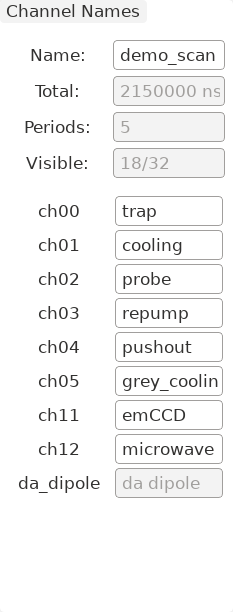
\includegraphics[width=0.78\textwidth]{assets/frontend_gui_names.png}
  \caption{Edit 页最左侧的 Channel Names 面板。顶部是 Name / Total / Periods / Visible 四个带标签的字段，下面是逐通道的两列：左边只读的物理引脚名（如 \pyapi{M17}），右边可编辑的显示名（如 \pyapi{cooling}）。}
\end{figure}

\subsection{这块面板是什么、在哪里}

Channel Names 面板是 Edit 页\tfocus{最左边}的一张白色、带标题的卡片，标题就写着 \pyapi{Channel Names}。它的职责只有两件事：一是显示并让你修改整条脉冲序列的\tfocus{身份信息}（名字、总时长、周期数、可见通道数），二是为每一条\tfocus{通道}提供两个名字——一个是硬件上固定的物理引脚名（只读），一个是你自己起的、好记的显示名（可改）。

\begin{notebox}[先记住一句话]
这块面板里能真正\tfocus{改变硬件行为}的东西非常少。除了最上面的 \pyapi{Name} 是给整个文件起名，下面每条通道右边的“显示名”\tfocus{只改怎么显示、不改硬件}。其余字段全部是\tfocus{只读}的、自动算出来的，看就行，改不了也不用改。
\end{notebox}

\subsection{顶部信息区：Name / Total / Periods / Visible}

面板顶部是四行，每行左边是一个标签，右边是对应的值。它们一行一个字段，从上到下排列。除了 \pyapi{Name} 可以编辑，其余三个都是\tfocus{只读}的——也就是说你点进去也敲不动，它们的数值会随着你在别处的修改\tfocus{自动实时更新}。

\begin{description}
\item[Name（名字）] 这是\tfocus{唯一可编辑}的顶部字段，是一个普通的文本输入框，里面装着这条脉冲序列的名字。
  \begin{itemize}
  \item \tfocus{作用}：这个名字有两个真实用途——保存时它会成为输出的 \filepath{.json} 文件名；画预览图时它会成为图的标题。所以起一个有意义的名字，以后翻文件、看图都省事。
  \item \tfocus{接受什么}：任意文本。建议只用字母、数字、下划线，避免空格和 \pyapi{/}、\pyapi{\textbackslash}、\pyapi{:} 这类在文件名里非法或容易出问题的字符。
  \item \tfocus{填了会怎样}：你敲进去的文字会被记住，下次保存就用它当文件名，下次画图就用它当标题。
  \item \tfocus{常见坑}：如果名字里带了路径分隔符或非法字符，保存成文件这一步可能会出错或生成奇怪的文件名；两条序列起了同一个名字，保存时后者会覆盖前者的同名文件。
  \item \tfocus{小技巧}：把关键参数编进名字里，比如 \pyapi{cooling\_scan\_2150us}，这样不打开文件、光看文件名就知道它是干嘛的。
  \end{itemize}

\item[Total（总时长）] \tfocus{只读}。显示整条序列的总持续时间，带单位 \pyapi{ns}（纳秒），例如 \pyapi{2150000 ns}。
  \begin{itemize}
  \item \tfocus{作用}：让你一眼看到这条序列从头到尾跑多久。它是把\tfocus{所有周期的时长加起来}得到的。
  \item \tfocus{怎么变}：你改不了这个框本身。但只要你在别处改了任何一个周期的时长，这里的 Total 会\tfocus{立刻重新计算并刷新}，不需要你手动按任何按钮。
  \item \tfocus{常见坑}：新手常以为可以直接在这里打一个目标总时长——不行，它是算出来的结果，不是输入。想改总时长，得去改各个周期的时长。
  \item \tfocus{小技巧}：把它当成一个\tfocus{校验仪表}。如果你心里预期总长是 2.15 ms，而这里显示的 \pyapi{ns} 数对不上，那多半是某个周期时长填错了，回去逐个核对。
  \end{itemize}

\item[Periods（周期数）] \tfocus{只读}。显示这条序列里\tfocus{周期}的数量，例如 \pyapi{5}。
  \begin{itemize}
  \item \tfocus{作用}：告诉你这条序列被切成了几个时间段（周期）。每个周期是序列在时间轴上的一段，有自己的时长和各通道的开关状态。
  \item \tfocus{怎么变}：同样是自动的。你在别处增加或删除周期，这个数字会跟着加减。
  \item \tfocus{常见坑}：它和 \pyapi{Visible} 是两回事——\pyapi{Periods} 数的是\tfocus{时间上的段数}，\pyapi{Visible} 数的是\tfocus{通道（行）的条数}，别混淆。
  \item \tfocus{小技巧}：当预览图看起来段数不对时，先瞄一眼这个数字，能快速确认你到底建了几个周期。
  \end{itemize}

\item[Visible（可见通道数）] \tfocus{只读}。以 \pyapi{已显示/总数} 的形式显示通道计数，例如 \pyapi{18/32}。
  \begin{itemize}
  \item \tfocus{作用}：斜杠左边是当前\tfocus{正在显示}的通道数，右边是\tfocus{全部}通道数。\pyapi{18/32} 表示一共有 32 条通道，目前面板上显示了其中 18 条。
  \item \tfocus{为什么会少显示}：硬件可能有很多条通道，但你这条实验通常只关心一部分；界面会把无关的通道隐藏起来，让你专注在用到的那些上。
  \item \tfocus{常见坑}：如果你觉得“某条通道怎么找不到了”，先看这里——如果左边数字小于右边，说明确实有通道被隐藏了，它不是消失了，只是没显示。
  \item \tfocus{小技巧}：把它当作一个\tfocus{完整性检查}。右边的总数应当等于你硬件实际的通道总数；左边的数应当等于下面逐通道列表里你能数出来的行数。
  \end{itemize}
\end{description}

\subsection{逐通道两列：左边只读引脚名 + 右边可编辑显示名}

顶部信息区下面，是\tfocus{一条通道一行}的列表，只列出当前可见的那些通道（也就是 \pyapi{Visible} 左边那个数那么多行）。每一行有两列：左边是硬件给定的、改不了的物理名字；右边是一个你可以随便改的、好记的显示名输入框。

\begin{description}
\item[左列：raw 标签（物理引脚名，只读）] 每行最左边是一个\tfocus{只读}标签，显示这条通道对应的\tfocus{物理封装引脚名}。
  \begin{itemize}
  \item \tfocus{它显示什么}：如果软件知道这条通道接到了板子上的哪个引脚（来自板卡的 XDC 约束文件），就显示那个引脚名，例如 \pyapi{M17}；如果不知道，就退而显示内部名 \pyapi{chNN}，例如 \pyapi{ch00}。
  \item \tfocus{为什么只读}：这是硬件接线决定的事实，不是你能在软件里改的。它代表“第几号物理输出”，改它没有意义，所以软件不让你动。
  \item \tfocus{名字太长会怎样}：当引脚名太长、一行放不下时，界面会用 \pyapi{...} 把它截断显示；\tfocus{完整文本会放进鼠标悬停提示（tooltip）}里。
  \item \tfocus{一个永远的保底}：不管左边显示的是引脚名还是被截断的文字，\tfocus{完整的内部名 \pyapi{chNN} 始终能在该标签的 tooltip 里看到}。所以你随时可以把鼠标停在上面，确认这到底是第几号通道。
  \item \tfocus{常见坑}：不要把这个只读的 \pyapi{M17} 当成可以重命名的东西去双击——它不会进入编辑状态。想起别名，请用它右边那个框。
  \item \tfocus{小技巧}：当你需要把界面上的某条通道和实际接线、和 FPGA 比特位对上号时，悬停看 tooltip 里的 \pyapi{chNN}，这是最可靠的对照方式。
  \end{itemize}

\item[右列：display-label 输入框（显示名，可编辑）] 每行右边是一个\tfocus{可编辑}的文本框，让你给这条通道起一个人类好记的名字，例如 \pyapi{cooling} 或 \pyapi{da\_dipole[0]}。
  \begin{itemize}
  \item \tfocus{作用}：纯粹是\tfocus{显示用}的别名。你填的名字会出现在界面的各处标签上，以及预览图的 y 轴上，让你看图、找通道时一眼认出谁是谁。
  \item \tfocus{关键事实——它不改硬件}：这个显示名\tfocus{只影响“怎么显示”，绝不改变硬件的比特位顺序}。也就是说，无论你把第 0 号通道叫 \pyapi{cooling} 还是叫 \pyapi{laser\_A}，它在 FPGA 里仍然是同一根输出、同一个比特位。改名只换标签，不换接线。
  \item \tfocus{接受什么}：任意文本，可以带方括号和下标风格的写法，例如 \pyapi{da\_dipole[0]}，方便你给同类通道编号。
  \item \tfocus{填了会怎样}：你敲完之后，界面上引用这条通道的地方、以及预览图 y 轴上对应的那一行，都会换成你起的新名字。
  \item \tfocus{常见坑}：千万别误以为“把两条通道的显示名对调，就能交换它们的硬件输出”——不会的，硬件顺序由比特位决定，显示名只是贴在外面的标签。还有，给两条通道起完全一样的显示名虽然不报错，但看图时容易把自己搞糊涂。
  \item \tfocus{小技巧}：用统一的命名规则（比如冷却光统一叫 \pyapi{cooling}、偶极阱用 \pyapi{da\_dipole[0]}、\pyapi{da\_dipole[1]}），预览图 y 轴会立刻变得清爽好读，排查实验问题时事半功倍。
  \end{itemize}
\end{description}

\subsection{对齐契约：三列同一行、一起滚动}

这块面板看起来简单，但它和它\tfocus{右边那块}面板之间有一个重要的、刻意保证的\tfocus{对齐约定}，新手了解一下能少很多困惑。

\begin{description}
\item[同一条通道，三样东西在同一行] 对任意一条通道来说，它在本面板里的\tfocus{左列只读引脚名}、它在右边相邻面板里的\tfocus{delay（延时）框}、以及它在周期区里的\tfocus{第一个周期的勾选框}，三者\tfocus{处在同一行上}——它们的\tfocus{垂直中心是对齐的}。
\item[三列一起上下滚动] 这三列在垂直方向上是\tfocus{联动滚动}的：你往下滚动通道列表时，引脚名、delay 框、勾选框会\tfocus{一起同步移动}，绝不会出现“名字滚到下面去了、它的延时框却还停在上面”这种错位。
\end{description}

\begin{notebox}[这个对齐为什么重要]
因为你经常需要\tfocus{横着读一整行}：先在最左边认出这是哪条通道（看引脚名或显示名），再顺着同一行往右看它的延时是多少、它在第一个周期里开没开。正因为三列严格对齐、一起滚动，你才可以放心地“一行从左读到右”，不用担心读串行。如果哪天你觉得名字和延时框对不上，那通常意味着界面出了渲染问题，而不是这条通道的设定真的错位了。
\end{notebox}

\section{Edit 页 — Delay / Scan 面板与扫描圆点（逐控件详解）}

本节面向\tfocus{从未见过本软件界面}的新用户，逐个控件讲解 Edit（编辑）页中第二个面板——\tfocus{Delay / Scan（延迟 / 扫描）面板}。它是从左数第二张白色带标题的卡片，标题写着 \pyapi{Delay / Scan}。这张卡片管两件事：一是给每个通道设置固定的\tfocus{延迟（delay）}，用来补偿线缆和设备的固有时延；二是把某些数值字段\tfocus{绑定成扫描变量}，让一次实验自动扫过一组取值。下面先看顶部的一组全局控件，再看每个通道一行里的各个控件，最后专门讲贯穿全软件的\tfocus{扫描圆点（scan dot）}。

\begin{figure}[htbp]
  \centering
  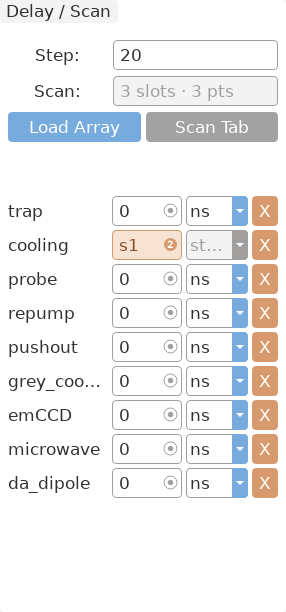
\includegraphics[width=0.92\textwidth]{assets/frontend_gui_delay.png}
  \caption{Delay / Scan 面板的整体外观。顶部是 Step / Scan 只读信息与 Load Array、Scan Tab 两个按钮；下方每个通道一行，依次是延迟输入框（右侧嵌着扫描圆点）、单位下拉框和一个 X 隐藏按钮。}
\end{figure}

\subsection{顶部信息区：Step 与 Scan（两个只读显示）}

面板顶部有两条\tfocus{只读}信息。只读的意思是它们只用来\tfocus{显示状态}，你无法直接在上面打字修改；它们的内容会随着你在别处的操作自动更新。

\begin{description}
\item[Step] 作用：显示当前测序器（sequencer）的\tfocus{时钟节拍长度}，也就是硬件最小的时间分辨率。默认值是 \pyapi{20 ns}，对应 50\,MHz 的时钟（一个周期 = 1 / 50\,MHz = \pyapi{20 ns}）。它接受的不是你的输入，而是反映系统设定。关键影响：你在本软件里输入的\tfocus{任何时间量}（例如某个通道的延迟）都会被自动\tfocus{量化（quantize）}成 Step 的整数倍。也就是说，如果 Step 是 \pyapi{20 ns}，你输入 \pyapi{30 ns}，系统会把它对齐到最接近的 \pyapi{20 ns} 的倍数（如 \pyapi{20 ns} 或 \pyapi{40 ns}）。常见的坑：新手会奇怪“为什么我填的数被改了”——这正是量化在起作用，不是 bug。实用提示：先在心里把目标时间换算成 Step 的整数倍再填，所见即所得，省去反复试。

\item[Scan] 作用：用一行简短文字\tfocus{汇总}当前已经绑定的扫描槽（slot）数量和扫描点数，形如 \pyapi{3 slots · 3 pts}，意思是“当前绑定了 3 个扫描槽、扫描表里有 3 个扫描点”。它接受的同样不是输入，而是自动统计。点击或输入：你不能在这里点或改，它只随你在各处绑定/解绑扫描圆点、或载入扫描表而变化。常见的坑：当这里显示 \pyapi{0 slots} 时，说明你还没有绑定任何扫描变量，这次运行就是一次普通的单点序列，而不是扫描。实用提示：每次绑定完圆点后瞄一眼这里，确认 slots 数和 pts 数都符合你的预期，是排查“为什么没在扫”的最快办法。
\end{description}

\subsection{顶部按钮：Load Array 与 Scan Tab}

\begin{description}
\item[Load Array 按钮] 作用：打开一个\tfocus{文件选择对话框}，从磁盘载入一份\tfocus{扫描表（scan table）}文件。可接受的文件类型是 \pyapi{.npy} / \pyapi{.csv} / \pyapi{.txt}。文件的格式约定非常重要：\tfocus{每一行代表一个扫描点，每一列代表一个已绑定的扫描槽}。点击后会发生什么：弹出系统文件对话框，你选中文件后，表里的数值就会被读进来，作为各扫描点上各个槽的取值。常见的坑：文件\tfocus{列数必须和当前绑定的槽数一致}——如果你绑定了 3 个槽，文件却只有 2 列（或多了一列），数据就对不上；另外别把行列搞反了（行=点、列=槽）。实用提示：如果你不想手写文件，可以改用 Scan Tab 页\tfocus{用代码生成}扫描表；Load Array 更适合从外部仪器或脚本导出的现成数据。

\item[Scan Tab 按钮] 作用：一键\tfocus{切换到 Scan（扫描）页}。Scan 页是你\tfocus{用代码来构造扫描表}的地方——在那里你针对每个槽（用 \pyapi{s0}、\pyapi{s1} 等变量名）写表达式，生成每个扫描点的取值。点击后会发生什么：界面从当前 Edit 页跳到 Scan 页，方便你在“绑定字段”和“填写扫描数值”两件事之间来回。常见的坑：先在 Edit 页用扫描圆点把字段\tfocus{绑定}成槽（这一步决定有几个槽、它们对应哪些字段），再去 Scan 页填这些槽的取值；顺序反了会发现没有槽可以写。实用提示：把 Scan Tab 当成“写完延迟和绑定后，去填扫描数值”的快捷入口。
\end{description}

\subsection{每个通道一行：延迟输入框（delay field）}

面板下方是\tfocus{逐通道}的若干行，每个通道占一行。每行最主要的控件是\tfocus{延迟输入框}，它是一个单行文本框，默认显示 \pyapi{0}。

\begin{description}
\item[延迟输入框] 作用：给\tfocus{这一个通道的所有边沿}加上一个\tfocus{固定的时间偏移}，用来补偿线缆长度、设备响应等带来的固有时延。可接受的值：一个时间数值，\tfocus{可正可负}——正值把该通道的所有上升/下降沿整体\tfocus{往后推}，负值整体\tfocus{往前提}。它\tfocus{不会改变任何周期（period）的时长}，只是把该通道的边沿整体平移。输入后会发生什么：该数值会被按 Step \tfocus{量化}成节拍的整数倍（见上文 Step），然后该通道在时间轴上的所有跳变都按这个偏移挪动。常见的坑：（1）以为延迟会拉长或缩短脉冲——不会，它只平移边沿，脉冲宽度和周期长度不变；（2）忘了它是\tfocus{按通道}独立的，改了 A 通道不影响 B 通道。实用提示：先用示波器量出某条线相对基准慢了多少 ns，把这个值（取正补偿滞后）填进去即可；负延迟同样合法，适合让某通道\tfocus{提前}触发。
\end{description}

\subsection{每个通道一行：单位下拉框与 X 隐藏按钮}

\begin{description}
\item[单位下拉框（ns / us / ms / s）] 作用：选择该行延迟数值的\tfocus{时间单位}。可选项是 \pyapi{ns}、\pyapi{us}、\pyapi{ms}、\pyapi{s} 四个。点击后会发生什么：下拉展开，选中某个单位后，左边输入框里的数字就按这个单位解释（例如填 \pyapi{1} 配 \pyapi{us} 等于 1 微秒）。常见的坑：单位选错会让延迟差出几个数量级（把 \pyapi{us} 当成 \pyapi{ns} 会小 1000 倍）；另外注意最终值仍要被 Step 量化，所以填一个比 Step 还小的单位组合可能被对齐成 \pyapi{0}。实用提示：日常脉冲多用 \pyapi{ns} 或 \pyapi{us}；填完先看一眼 Step 量化后是不是你要的值。

\item[X 按钮（隐藏通道）] 作用：把该通道从表里\tfocus{隐藏}，让界面更清爽。点击后会发生什么：这一行从 Delay / Scan 表里消失，该通道被移到\tfocus{隐藏列表}中。它去哪了：底部的 \pyapi{Channels}（通道）卡片会记录被隐藏的通道，你可以从那里把它\tfocus{重新调出来}。常见的坑：以为 X 是“删除/禁用通道”——它只是\tfocus{视觉上隐藏}，不会改动该通道的脉冲内容；找不回来时别新建，去底部 Channels 卡找。实用提示：把当前实验用不到的通道隐藏起来，可以让一长串通道里真正关心的几行更醒目、对齐更易读。
\end{description}

\subsection{扫描圆点（scan dot）——把字段变成扫描变量}

\tfocus{扫描圆点}是贯穿整个软件的关键控件：它不仅出现在这里的\tfocus{延迟（delay）}字段右侧，也出现在周期的\tfocus{时长（duration）}字段和\tfocus{DAC 值}字段上。它嵌在输入框的\tfocus{右边缘}，外形和行为都像 spinbox（数值微调框）那个上下小按钮，\tfocus{垂直居中}。它的核心作用，是把一个普通的数值字段“升级”为一个会在实验里被自动扫过的\tfocus{扫描槽（slot）}。

\begin{figure}[htbp]
  \centering
  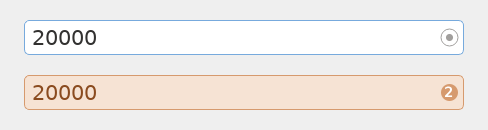
\includegraphics[width=0.52\textwidth]{assets/frontend_gui_dot.png}
  \caption{扫描圆点的两种状态。左：未绑定——空心灰色圆环加一个小小的中心点；右：已绑定——实心橙色圆点，里面显示该槽的 1 起编号（\pyapi{s0} 显示 “1”），同时字段变成淡橙底、深橙字的只读样式。}
\end{figure}

\begin{description}
\item[未绑定时的外观] 一个\tfocus{空心灰色圆环}，中间有一个很小的中心点。看到这个样子，说明该字段还是普通可编辑的数值，没有参与扫描。

\item[点击一次：绑定（bind）] 作用：把该字段绑定到一个扫描槽。点击后会发生三件事：（1）字段变成\tfocus{橙色样式}——淡橙色背景、深橙色文字，并变为\tfocus{只读}（你不能再直接在框里打字，因为它的值现在由扫描表决定）；（2）圆点变成一个\tfocus{实心橙色圆点}，里面显示该槽的\tfocus{从 1 起的编号}——槽 \pyapi{s0} 显示 “1”，\pyapi{s1} 显示 “2”，以此类推；（3）字段里原本存的数值被\tfocus{改写成一个符号表达式} \pyapi{s0} / \pyapi{s1} ……，表示“此处的值取自对应扫描槽”。

\item[再点一次：解绑（unbind）] 作用：把字段从扫描槽上解开，恢复成普通可编辑数值。贴心之处：当你\tfocus{再次绑定同一个字段}时，之前为它在扫描表里填过的那些数值会\tfocus{被记住并恢复}，不用重填。

\item[这等价于哪条 API] 这个圆点就是图形界面里对应的一次 API 调用 \pyapi{state.bind_field(kind, target)}——也就是说，鼠标点圆点和在代码里调用 \pyapi{bind_field} 是同一件事的两种入口。

\item[编号与重新编号（重要的坑）] 槽按\tfocus{绑定顺序}依次命名为 \pyapi{s0}、\pyapi{s1}、\pyapi{s2} ……。如果你\tfocus{解绑中间的一个槽}，它后面的槽会\tfocus{自动重新编号}向前补位——因为这个编号\tfocus{就是表达式里用的 s 变量}本身。常见的坑：你在 Scan 页或某个表达式里写死了 \pyapi{s2}，结果解绑了前面的槽，原来的 \pyapi{s2} 变成了 \pyapi{s1}，含义就跟着变了。实用提示：尽量\tfocus{先把所有要扫的字段绑定齐}再去写扫描表达式；若必须中途解绑，回头核对一遍各表达式里的 s 编号是否还指向你想要的字段，并瞄一眼顶部 Scan 汇总确认槽数正确。
\end{description}

\begin{notebox}[一句话记住扫描圆点]
灰色空心环 = 普通数值；点一下变\tfocus{橙色实心带编号} = 这个字段交给扫描槽 \pyapi{s$n$} 自动扫；再点一下还原，且\tfocus{记得}你之前填的扫描值。编号即 s 变量，解绑中间槽会让后面的槽\tfocus{整体前移}。
\end{notebox}

\section{Edit 页 — period 卡片与 DAC 行（逐控件详解）}

本节面向\tfocus{从未见过本软件界面}的新用户，逐个讲清楚 Edit 页里一张「period 卡片」上的每一个控件。读完你应该能独立看懂、填写、并安全地编辑一段脉冲时序，而不需要旁人指导。

\begin{figure}[htbp]
  \centering
  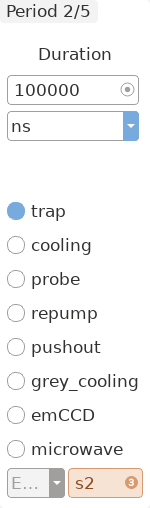
\includegraphics[width=0.62\textwidth]{assets/frontend_gui_period.png}
  \caption{Edit 页中一张典型的 period 卡片，从上到下依次是位置标签、Duration 输入框（带嵌入式扫描圆点）与单位下拉、若干通道复选框，以及每条模拟总线一行的 DAC（mode 下拉 + value 输入框）。}
\end{figure}

\subsection{先理解：period 卡片是「时间轴」，不是表格}

在 Edit 页里，每一个 period（时间段）都被画成一张\tfocus{白色卡片}。这些卡片在一条\tfocus{可以横向滚动的时间轴}上从左到右一字排开——请把它们想象成一条被切成若干段的时间带，而\tfocus{不是}一张可以随意填格子的二维表格。

\begin{description}
\item[作用] 一张卡片代表「一段连续的时间」。在这段时间里，每条数字通道要么一直是高电平、要么一直是低电平；每条模拟总线（DAC）保持某个码值或做某种变化。整条实验时序就是这些时间段一段接一段拼起来的。
\item[卡片之间的顺序] 卡片从左到右的排列顺序\tfocus{就是}实际执行的先后顺序。最左边的卡片先发生，往右依次执行。
\item[点击或拖动后会发生什么] \tfocus{拖动卡片可以重新排序 period}。把一张卡片拖到另一张前面或后面，时序里这段时间的发生位置就跟着改变。这是调整实验流程顺序最直接的方式。
\item[常见坑] 因为是时间轴而不是网格，不要指望「上下对齐的格子」有某种行列关系——真正有意义的只有\tfocus{左右顺序}。如果时间轴很长，记得用横向滚动条往右翻，后面可能还有卡片没显示出来。
\item[实用提示] 在动手填数值之前，先从左到右快速浏览一遍所有卡片，建立「这段实验先做什么、再做什么」的整体印象，再去抠每个控件的细节，会高效很多。
\end{description}

\subsection{位置标签（卡片顶部）}

每张卡片最上方有一行\tfocus{位置标签}，例如 \pyapi{Period 2 / 5}。

\begin{description}
\item[作用] 它告诉你「这是第几张卡片，一共有几张」。\pyapi{Period 2 / 5} 表示当前这张是第 2 个 period，整条时序总共有 5 个 period。
\item[接受什么值] 这是一个\tfocus{只读的显示标签}，不是输入框，你不能点进去改它。它的数字会随着你增删、拖动 period 自动更新。
\item[点击后会发生什么] 它本身不响应编辑。它的价值在于「定位」——当你在一长串卡片里来回滚动时，靠这个标签快速确认自己正在看第几段。
\item[常见坑] 如果你拖动卡片重新排序，标签里的编号会立刻重排（原来的「Period 2」可能变成「Period 3」）。所以不要用编号去记忆某段的内容，内容才是它的身份。
\item[实用提示] 当总数（斜杠后的数字）和你预期的 period 数量不一致时，说明你可能多加或漏加了一段，借这个标签能第一时间发现。
\end{description}

\subsection{Duration 输入框（带嵌入式扫描圆点）}

紧接位置标签下面是 \tfocus{Duration} 字段：一个文本输入框，右侧嵌着一个小小的\tfocus{扫描圆点（SCAN DOT）}，就像数字微调框右边那个按钮一样。

\begin{description}
\item[作用] 它决定「这一段时间持续多久」，也就是这个 period 的长度。
\item[接受什么值] 通常直接填一个\tfocus{数字}（配合右边的单位下拉决定它是 ns/us/ms/s）。除此之外，它还能填一个\tfocus{符号表达式}，例如 \pyapi{s0}、或者 \pyapi{s1+20} 这样的式子——这用于「仿射扫描模板」，让这一段的时长随扫描槽的取值而变化。要填符号表达式时，必须把右边单位切到 \pyapi{str (ns)}。
\item[嵌入式扫描圆点] 输入框右侧那个圆点用来把这个 Duration 字段\tfocus{绑定到一个扫描槽}。绑定后该字段会以橙色高亮、显示成 \pyapi{s0}/\pyapi{s1} 之类的符号，表示「这段时长不是固定的，会在扫描的各个点上取不同的值」。再次点击圆点可以解除绑定、恢复成普通数值。
\item[点击或输入后会发生什么] 填入一个数字并配好单位后，这段时间的实际长度立即按该数值生效；如果填的是符号、或点了扫描圆点，这一段就变成可扫描的，实际时长在运行扫描时由对应扫描槽逐点提供。
\item[常见坑] \tfocus{时长为 0 是不允许的}——一个 period 必须有正的持续时间，填 0 会被拒绝。另外，想用 \pyapi{s0}、\pyapi{s1+20} 这种符号表达式时，单位\tfocus{必须}选 \pyapi{str (ns)}；如果单位还停在 ns/us 等数字单位上而框里写了符号，就会对不上。
\item[实用提示] 表达式里只能使用 \pyapi{s0}、\pyapi{s1}…… 这类扫描槽符号（按槽编号从 0 开始），\pyapi{s1+20} 的含义是「在第 1 号扫描槽的值上再加 20 ns」。需要「以某个扫描值为基准、固定偏移一点」时，这种写法非常顺手。
\end{description}

\subsection{单位下拉（Duration 旁边）}

Duration 输入框旁边有一个\tfocus{单位下拉框（combo）}。

\begin{description}
\item[作用] 它决定 Duration 框里那个数值按什么时间单位解释。
\item[接受什么选项] 共有 \pyapi{ns} / \pyapi{us} / \pyapi{ms} / \pyapi{s} 四个数字单位，外加一个特殊项 \pyapi{str (ns)}。前四个用于普通的固定时长；\pyapi{str (ns)} 专门用于\tfocus{符号化/可扫描}的时长，让 Duration 框接受像 \pyapi{s0} 或 \pyapi{s1+20} 这样的表达式（其数值按 ns 解释）。
\item[点击后会发生什么] 切换单位会改变 Duration 框里数字的量纲。例如同样填 \pyapi{100}，选 \pyapi{ns} 是 100 纳秒，选 \pyapi{us} 就是 100 微秒，相差一千倍。
\item[常见坑] 最容易出错的就是\tfocus{单位和内容不匹配}：想写符号表达式却没把单位切到 \pyapi{str (ns)}；或者本想填微秒却把单位留在了 ns（导致时间短了一千倍）。每次改完 Duration，习惯性扫一眼单位框是否正确。
\item[实用提示] 当你打算把这一段时长拿去扫描、或写成依赖扫描槽的表达式时，\tfocus{先}把单位切到 \pyapi{str (ns)}，再去填表达式或点扫描圆点，顺序对了就不会出现「符号被当成普通数字」的尴尬。
\end{description}

\subsection{通道复选框（每条可见通道一个）}

卡片中段是一排\tfocus{复选框}，每一条当前可见的数字通道对应一个复选框。

\begin{description}
\item[作用] 它控制「在这一段时间里，这条通道是高还是低」。\tfocus{勾选 = 该通道在本 period 内为高电平（HIGH）}；\tfocus{不勾 = 低电平（low）}。
\item[接受什么值] 只有「勾 / 不勾」两种状态，没有中间态。
\item[点击后会发生什么] 勾上某通道，本段时间里这条线就被拉高；取消勾选则保持低。整段时间内电平不变——要让一条通道在某时刻翻转，就靠相邻 period 之间该复选框勾选状态的不同来实现。
\item[标签被省略的情况] 通道标签如果太长，会被用省略号 \pyapi{...} 截断显示；\tfocus{完整名字在鼠标悬停的 tooltip 里}。所以看不清全名时，把鼠标停在标签上稍等即可看到完整通道名。
\item[常见坑] 因为标签会被省略，不同通道的截断结果可能看起来很像，容易勾错行。下手前最好靠 tooltip 确认这一行到底是哪条通道。
\item[实用提示] 把「这条通道在哪几段为高」想成在时间轴上画一条方波：相邻卡片勾选状态相同就是电平保持，状态变化的地方就是一个上升沿或下降沿。顺着卡片从左到右看这一列复选框，就能一眼读出该通道的整个波形。
\end{description}

\subsection{DAC（模拟总线）行 — mode 下拉}

卡片下部，\tfocus{每一条模拟总线（DAC）}各占一行，例如 \pyapi{da_dipole}。每行由两个控件组成：一个 mode 下拉 + 一个 value 输入框。先看 mode 下拉。

\begin{description}
\item[作用] mode 下拉决定「这一段时间里，这条 DAC 的值如何变化」。
\item[接受什么选项] 三个选项：\pyapi{Edge} / \pyapi{Ramp} / \pyapi{Hold}。
\item[各选项的含义]
  \begin{description}
  \item[\pyapi{Edge}] 在本 period \tfocus{开始的瞬间直接跳到} value 框里写的那个值，然后整段保持该值。适合需要在段首做阶跃变化的场合。
  \item[\pyapi{Ramp}] 在本段时间内\tfocus{从上一段的值线性渐变到}本段 value 框里的目标值。适合做平滑扫频/缓变控制。
  \item[\pyapi{Hold}] \tfocus{保持上一段的值不变}（本段不做任何改变），此时这一行的 value 等于沿用之前的码值。
  \end{description}
\item[点击后会发生什么] 选 \pyapi{Edge} 会让 value 框里的数立刻在段首生效；选 \pyapi{Ramp} 会让输出在这一整段里从「前值」滑到「本段值」；选 \pyapi{Hold} 则忽略本段 value、延续旧值。
\item[常见坑] \pyapi{Ramp} 的起点是「上一段结束时的值」，不是 0，也不是本段框里的数——如果你忘了前一段的值是多少，渐变的起点可能和预期不同。\pyapi{Hold} 模式下你在 value 框里改数往往不起作用，因为它本就保持旧值。
\item[实用提示] 想要一个干净的阶跃，用 \pyapi{Edge}；想要一条斜坡，把斜坡终点写进本段 value 并选 \pyapi{Ramp}，同时确认前一段已经把起点值设好；只想「这段别动这条 DAC」就选 \pyapi{Hold}。
\end{description}

\subsection{DAC（模拟总线）行 — value 输入框（带嵌入式扫描圆点）}

每条 DAC 行的第二个控件是 \tfocus{value 输入框}，同样在右侧嵌了一个\tfocus{扫描圆点}。

\begin{description}
\item[作用] 它存放这条 DAC 在本段要输出的\tfocus{原始 10 位 DAC 码}。
\item[接受什么值] 一个 \pyapi{0} 到 \pyapi{1023} 之间的整数码值（10 位）。\tfocus{请注意这是原始码值，不是电压}——它直接对应 DAC 的数字输入，至于换算成多少伏，取决于硬件配置，本框里只管填码。
\item[嵌入式扫描圆点] 和 Duration 一样，右侧圆点用来把这个 value\tfocus{绑定到扫描槽}。一旦绑定，框里会显示成 \pyapi{s0}/\pyapi{s1} 之类的符号并\tfocus{变成橙色}，表示这条 DAC 的码值会在扫描的不同点上取不同值。再点一次圆点解除绑定、恢复成普通数字。
\item[点击或输入后会发生什么] 填入 0..1023 的整数后，配合本行 mode（\pyapi{Edge} 段首跳到该码 / \pyapi{Ramp} 渐变到该码）这个码值就会生效；点了扫描圆点绑定到扫描槽后，运行扫描时由对应槽逐点提供码值。
\item[常见坑] 值\tfocus{超出 0..1023} 是无意义的——10 位 DAC 只有这 1024 个码。另外别把它当电压填（比如填个「3.3」想表示 3.3 V 是错的，要填的是对应那个电压的整数码）。在 \pyapi{Hold} 模式下，这个框里的数通常不被采用，因为该模式沿用旧值。
\item[实用提示] \pyapi{1023} 是满量程最大码、\pyapi{0} 是最小码，中点大约在 \pyapi{512} 附近——心里有这个刻度，调码值时就能快速估出大概落在量程的什么位置。要扫描一条 DAC，直接点它 value 框右边的圆点绑定到扫描槽即可，绑定后橙色高亮会让你一眼看出「这条值是被扫描的」。
\end{description}

\begin{notebox}[一张卡片就是一段时间的全部状态]
把一张 period 卡片读完，你就知道了这段时间的「全部信息」：它持续多久（Duration + 单位）、每条数字通道是高还是低（复选框）、每条模拟总线输出什么码、怎么变（DAC 行的 mode + value）。整条实验时序，无非是把这样一张张卡片按时间轴从左到右拼接起来。\tfocus{时长不能为 0}、\tfocus{DAC 填的是 0..1023 的原始码而非电压}、\tfocus{拖动卡片即可重排顺序}——记住这三条，基本就不会在 Edit 页踩坑。
\end{notebox}

\section{Edit 页 — 底部 Control 与 Channels 控制条（逐按钮详解）}

Edit 页（脉冲编辑页）的最下方有一整条横向工具区，分成两张带标题的卡片：左侧是 \tfocus{Control}（运行与文件控制），右侧是 \tfocus{Channels}（通道显示控制）。如果你以前从没用过这个界面，可以把它想象成「磁带录音机的操作面板」：上半部分是你画脉冲波形的大画布，而这一条底部工具区就是控制「录、放、停、存、读」以及「让画面里显示哪些轨道」的按钮。下面对每一个按钮、每一个下拉框逐一讲清楚：它是干什么的、能接受什么值、点下去之后会发生什么、容易踩的坑，以及一个实用小提示。

\begin{figure}[htbp]
  \centering
  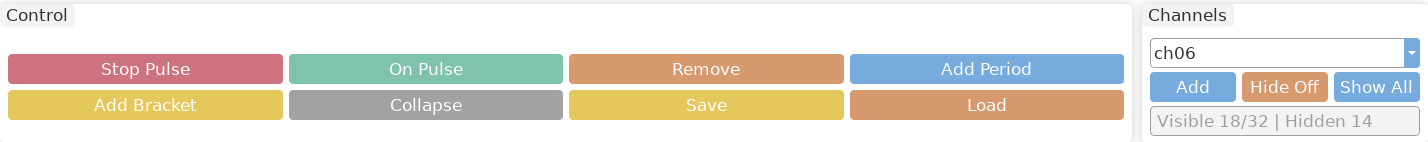
\includegraphics[width=\textwidth]{assets/frontend_gui_bottombar.png}
  \caption{Edit 页底部的两张控制卡片——左为 Control（8 个按钮，2 行 4 列），右为 Channels（下拉框 + 三个按钮 + 一个只读统计标签）。}
\end{figure}

\subsection{Control 卡片：运行控制按钮（Stop / On）}

Control 卡片一共有 8 个按钮，排成 2 行 4 列。最重要、也最需要先认识的是这两个带颜色的运行按钮。

\begin{description}
\item[Stop Pulse（红色）] \tfocus{作用}：把测序器（sequencer）切换到\tfocus{安全空闲状态}，也就是让所有硬件输出全部归零（所有通道变为低电平 0，DAC 总线也回到安全值）。\tfocus{接受什么}：这是一个纯动作按钮，没有任何输入框，直接点一下即可，没有参数可填。\tfocus{点下去会发生什么}：当前正在跑的脉冲序列会被立即叫停，FPGA 把全部输出拉到 0，进入待命。\tfocus{常见坑}：很多新手以为「关掉 GUI 窗口」就等于停止输出，其实不是——窗口关掉之后硬件可能仍按上一次的指令在跑。要真正让设备安静下来，必须显式点 Stop Pulse。\tfocus{实用提示}：把它当成「急停按钮」。只要你发现实验行为不对、激光或线圈有异常、或者准备离开设备，第一反应就是点这颗红色的 Stop Pulse，让一切归零，再慢慢排查。

\item[On Pulse（绿色）] \tfocus{作用}：这是「开始运行」按钮，而且它一颗按钮做两件事——先 \tfocus{prepare}（把当前编辑好的脉冲表上传/同步到测序器），\tfocus{然后}立刻 \tfocus{start}（启动它开始输出）。\tfocus{接受什么}：同样是纯动作按钮，无输入参数。\tfocus{点下去会发生什么}：你在画布上编辑的所有周期（period）、通道延时、扫描设置等会被编译并写进 FPGA，写完后序列马上开始跑。\tfocus{常见坑}：这里有一个对新手特别重要的事实——\tfocus{没有单独的「同步」或「上传」按钮}。不要去找一个「先上传再运行」的两步流程，因为 On Pulse 已经把上传和启动合并了。也就是说，每次你改完脉冲表想看效果，直接点 On Pulse 就会用\tfocus{最新}的内容重新上传并运行，旧内容不会残留。\tfocus{实用提示}：修改脉冲后无需任何额外操作，直接 On Pulse 即可让改动生效；如果你怀疑跑的还是旧版本，再点一次 On Pulse 强制重新上传即可。
\end{description}

\begin{notebox}[红绿配色的含义]
红色 = 让一切停下并归零（安全），绿色 = 上传并开始运行。养成「先看颜色再点」的习惯，可以避免在不该启动的时候误触发输出。
\end{notebox}

\subsection{Control 卡片：周期编辑按钮（Remove / Add Period / Add Bracket）}

这一组按钮用来增删脉冲表里的「周期（period）」结构，也就是改变时间线的骨架。

\begin{description}
\item[Remove] \tfocus{作用}：删除\tfocus{当前选中的（或最后一个）}周期。\tfocus{接受什么}：动作按钮，无输入。\tfocus{点下去会发生什么}：被选中的那个周期会从时间线上消失，后面的周期相应前移。\tfocus{常见坑}：如果你没有特意选中某个周期，它删除的是「最后一个」周期，所以可能删掉的并不是你以为的那一段；删之前先确认你选中的是哪一个。\tfocus{实用提示}：删错了不要慌——只要还没保存，可以再用 Add Period 补回一个空周期，再重新填内容；养成删除前先 Save 一次的习惯能让你随时回退。

\item[Add Period] \tfocus{作用}：在脉冲表末尾\tfocus{追加一个新的周期}。\tfocus{接受什么}：动作按钮，无输入。\tfocus{点下去会发生什么}：时间线右侧会多出一个新的（通常是空白/默认）周期卡片，你可以继续在里面设置各通道的开关与时长。\tfocus{常见坑}：新周期是加在\tfocus{末尾}的，不是插在你当前选中的位置中间；如果你需要在中间插入，得调整顺序或重新规划。\tfocus{实用提示}：搭建一个新序列时，先用 Add Period 把需要的周期数量一次性建够，再逐个填内容，比边建边填更不容易乱。

\item[Add Bracket] \tfocus{作用}：\tfocus{切换（toggle）}一个重复括号——也就是在一段连续的周期范围上加一个\tfocus{有限次的内层循环}（重复 ×N 次）。\tfocus{接受什么}：动作按钮（toggle 性质，再点一次可取消）。\tfocus{点下去会发生什么}：被括起来的那几个周期会作为一个内循环重复 N 次，而整张脉冲表本身\tfocus{仍然可以无限重复}（外层 ×∞）。换句话说，你能得到「整体永远循环、其中某几段又内部重复 N 次」的嵌套结构。\tfocus{常见坑}：要分清\tfocus{内层有限循环}和\tfocus{外层无限循环}是两回事——括号只控制内层那几段的重复次数，不影响整表是否一直跑下去。另外要注意，括号定义的是\tfocus{一段连续范围}，跨度选错会把不想重复的周期也圈进去。\tfocus{实用提示}：需要「先重复一组装载/冷却脉冲若干次，再继续后续步骤」时，Add Bracket 就是你要的工具；不需要时再点一次把它取消即可，因为它是可切换的。
\end{description}

\subsection{Control 卡片：Collapse（折叠左侧面板）}

\begin{description}
\item[Collapse] \tfocus{作用}：把左边的 \tfocus{Channel Names（通道名）} 面板和 \tfocus{Delay / Scan（延时/扫描）} 面板\tfocus{隐藏起来}，从而把腾出来的横向空间全部让给中间的周期时间线，让波形画布更宽、更好看。\tfocus{接受什么}：动作按钮（切换性质），无输入。\tfocus{点下去会发生什么}：左侧两块面板收起，时间线立刻变宽；同时这颗按钮的文字会从「Collapse」变成「\tfocus{Show Left}」，并且界面上会留下一个小小的存根（stub），让你随时能把面板再调回来。\tfocus{常见坑}：折叠之后通道名和延时编辑区暂时看不见了，新手容易以为「设置丢了」——其实只是被藏起来，数据都还在，点 Show Left（或那个小存根）就回来了。\tfocus{实用提示}：当你的序列周期很多、时间线被挤得很窄看不清细节时，先 Collapse 腾地方专心看波形；需要改通道名或延时时再 Show Left 调回来。
\end{description}

\subsection{Control 卡片：文件操作（Save / Load）}

\begin{description}
\item[Save] \tfocus{作用}：把当前脉冲保存成磁盘文件。\tfocus{接受什么}：动作按钮，无需在按钮上输入参数（实际文件名通过保存流程确定）。\tfocus{点下去会发生什么}：它会写出一个 \pyapi{.json} 脉冲文件，\tfocus{同时}附带写出一张预览图 \pyapi{.png}；并且\tfocus{如果当前存在扫描表（scan table）}，还会再写出一个 \pyapi{<name>_scan.npy} 数组文件。也就是说一次 Save 最多产出三个配套文件，方便你完整复现这次实验设置。\tfocus{颜色含义}：这颗按钮会变色来提示状态——当有\tfocus{未保存的修改}时它显示\tfocus{黄色}，当内容已经保存干净时它显示\tfocus{蓝色}。\tfocus{常见坑}：按钮上的文字\tfocus{始终是「Save」}，不会因为有未保存内容就变成别的字；「有没有未保存」是靠\tfocus{黄色}以及\tfocus{标题栏里的一个星号（star）}来表示的，别去找文字提示。\tfocus{实用提示}：把「Save 变成蓝色 + 标题栏星号消失」当作「已存盘」的可靠信号；运行前如果看到它还是黄色，说明你最新的改动还没落盘，建议先 Save 再 On Pulse，避免事后找不到这次用的是哪份配置。

\item[Load] \tfocus{作用}：从磁盘\tfocus{载入}一个脉冲 \pyapi{.json} 文件。\tfocus{接受什么}：动作按钮；会让你选择一个之前保存过的 \pyapi{.json}。\tfocus{点下去会发生什么}：选中的脉冲文件被读入，画布上的周期、通道、延时、扫描等设置会替换成文件里的内容。\tfocus{常见坑}：Load 会用文件内容\tfocus{覆盖}当前编辑区——如果你当前有未保存的改动（Save 还是黄色、标题栏有星号），载入前务必先 Save，否则改动会丢失。\tfocus{实用提示}：Save 与 Load 是一对——用统一的命名（让 \pyapi{.json}、\pyapi{.png} 预览图、\pyapi{_scan.npy} 同名成套）能让你日后一眼认出哪份配置对应哪次实验，复现和归档都更省心。
\end{description}

\begin{notebox}[一次 Save 到底产生几个文件？]
最少一个（\pyapi{.json} 脉冲本体），通常两个（再加一张 \pyapi{.png} 预览图）。只有当你设置了扫描表时才会有第三个 \pyapi{<name>_scan.npy}。看到 Save 变蓝、标题栏星号消失，就代表这一套都已经写好了。
\end{notebox}

\subsection{Channels 卡片：把隐藏通道调回来（下拉框 + Add）}

右侧的 Channels 卡片专门管「画面里显示哪些通道」，它不改变硬件输出，只改变\tfocus{你看到什么}。

\begin{description}
\item[隐藏通道 / DAC 总线 下拉框] \tfocus{作用}：这是一个下拉列表，里面列出当前\tfocus{被隐藏的}通道以及 DAC 总线，供你挑一个重新显示出来。\tfocus{接受什么}：从下拉项中选择一个条目（某个被藏起来的通道或某条总线）。\tfocus{点下去会发生什么}：仅仅是「选中」，此时还没真正显示——它只是告诉旁边的 Add 按钮「我要调回的是这一个」。\tfocus{常见坑}：光在下拉框里选好并不会让通道出现，必须再点 Add 才生效；如果下拉框是空的，说明当前没有被隐藏的通道可调回。\tfocus{实用提示}：先在下拉框里看一眼到底有哪些通道被藏了，这本身就是个快速排查「我的某个通道怎么不见了」的好办法。

\item[Add] \tfocus{作用}：把下拉框里\tfocus{当前选中}的那个通道/总线\tfocus{重新显示}出来。\tfocus{接受什么}：动作按钮，配合上面的下拉框使用。\tfocus{点下去会发生什么}：被选中的通道立刻回到时间线画布上，重新可见可编辑。\tfocus{常见坑}：注意这是「显示/隐藏」层面的操作，把通道调回来\tfocus{不会}改变它的脉冲内容，也不会改变硬件输出；别把它误解成「新增一个硬件通道」。\tfocus{实用提示}：配合下面的 Hide Off 一起用——先 Hide Off 把无关通道清掉，等需要某个特定通道时再用「下拉框选中 + Add」精准把它单独调回来。
\end{description}

\subsection{Channels 卡片：批量显示/隐藏（Hide Off / Show All）与统计标签}

\begin{description}
\item[Hide Off] \tfocus{作用}：\tfocus{隐藏所有「全程为关」的通道}——也就是那些在\tfocus{每一个周期里都处于关（低电平 0）}的通道，用来减少画面杂乱。\tfocus{接受什么}：动作按钮，无输入。\tfocus{点下去会发生什么}：凡是从头到尾都没被用到（始终是 0）的通道会从画布上消失，剩下的都是真正参与了这个序列的通道，画面立刻清爽很多。\tfocus{常见坑}：判断标准是「在\tfocus{每个}周期都为关」——只要某个通道在\tfocus{任意一个}周期里有过高电平，它就\tfocus{不会}被隐藏。所以如果你期望某条线被藏却没被藏，多半是它在某个周期里其实有输出。\tfocus{实用提示}：序列搭好后先点一下 Hide Off，能把几十条通道里真正在用的那几条凸显出来，审阅波形时效率高很多；想看全貌时再用下面的 Show All 还原。

\item[Show All] \tfocus{作用}：\tfocus{显示所有硬件通道}，把之前隐藏的全部调回来。\tfocus{接受什么}：动作按钮，无输入。\tfocus{点下去会发生什么}：所有硬件通道（无论之前是被 Hide Off 还是被单独隐藏的）一次性全部重新出现在画布上。\tfocus{常见坑}：通道一多画面会变得很密集、需要滚动，这是正常的；Show All 是「看全貌」用的，不适合长时间编辑细节。\tfocus{实用提示}：把 Hide Off 和 Show All 当成一对开关——\tfocus{Hide Off 聚焦、Show All 总览}。检查「是不是漏配了某个通道」时点 Show All，专注编辑时点 Hide Off。

\item[只读统计标签] \tfocus{作用}：这是一个\tfocus{不可编辑}的文字标签，实时显示当前的可见/隐藏统计，例如「\pyapi{Visible 18/32 | Hidden 14}」。\tfocus{接受什么}：它不接受任何输入，纯展示。\tfocus{点下去会发生什么}：什么都不会发生——它只是一面「仪表」，告诉你 32 条硬件通道里当前显示了 18 条、藏了 14 条。\tfocus{常见坑}：别试图点它或改它，它不是按钮也不是输入框。\tfocus{实用提示}：用它快速核对——比如你 Hide Off 之后看到「Visible 6/32」，就能立刻知道这个序列实际只用到了 6 条通道；数字和你的预期不符时，说明有通道被多配或漏配，值得回头检查。
\end{description}

\begin{notebox}[Channels 卡片只影响「显示」，不影响「输出」]
请牢记：Channels 卡片里的下拉框、Add、Hide Off、Show All 全部只改变\tfocus{画面上看到哪些通道}，丝毫不改变 FPGA 实际输出的脉冲。把一条通道藏起来，它在硬件上该高还是高、该低还是低；调出来也只是让你重新看见而已。真正改变运行行为的，是左边 Control 卡片里的 On Pulse / Stop Pulse。
\end{notebox}

The source confirms all the facts. Now I'll produce the LaTeX fragment.

\section{Preview 页与扫描高亮在预览里怎么显示（逐元素详解）}

Preview（预览）页是你在真正把脉冲发到 FPGA 之前，用来"用眼睛检查一遍"序列长什么样的地方。它把你在 Edit 页里搭好的周期表（period table）画成一张时间图：横轴是时间，纵轴是一行一行的通道。本节假设你\tfocus{从来没见过这个界面}，所以我们会把页面上每一个开关、按钮、每一种颜色的含义都讲透——它们各自\tfocus{有什么作用}、\tfocus{接受什么值}、\tfocus{点下去或切换后会发生什么}、\tfocus{常见的坑}，以及\tfocus{一个实用提示}。

\begin{figure}[htbp]
  \centering
  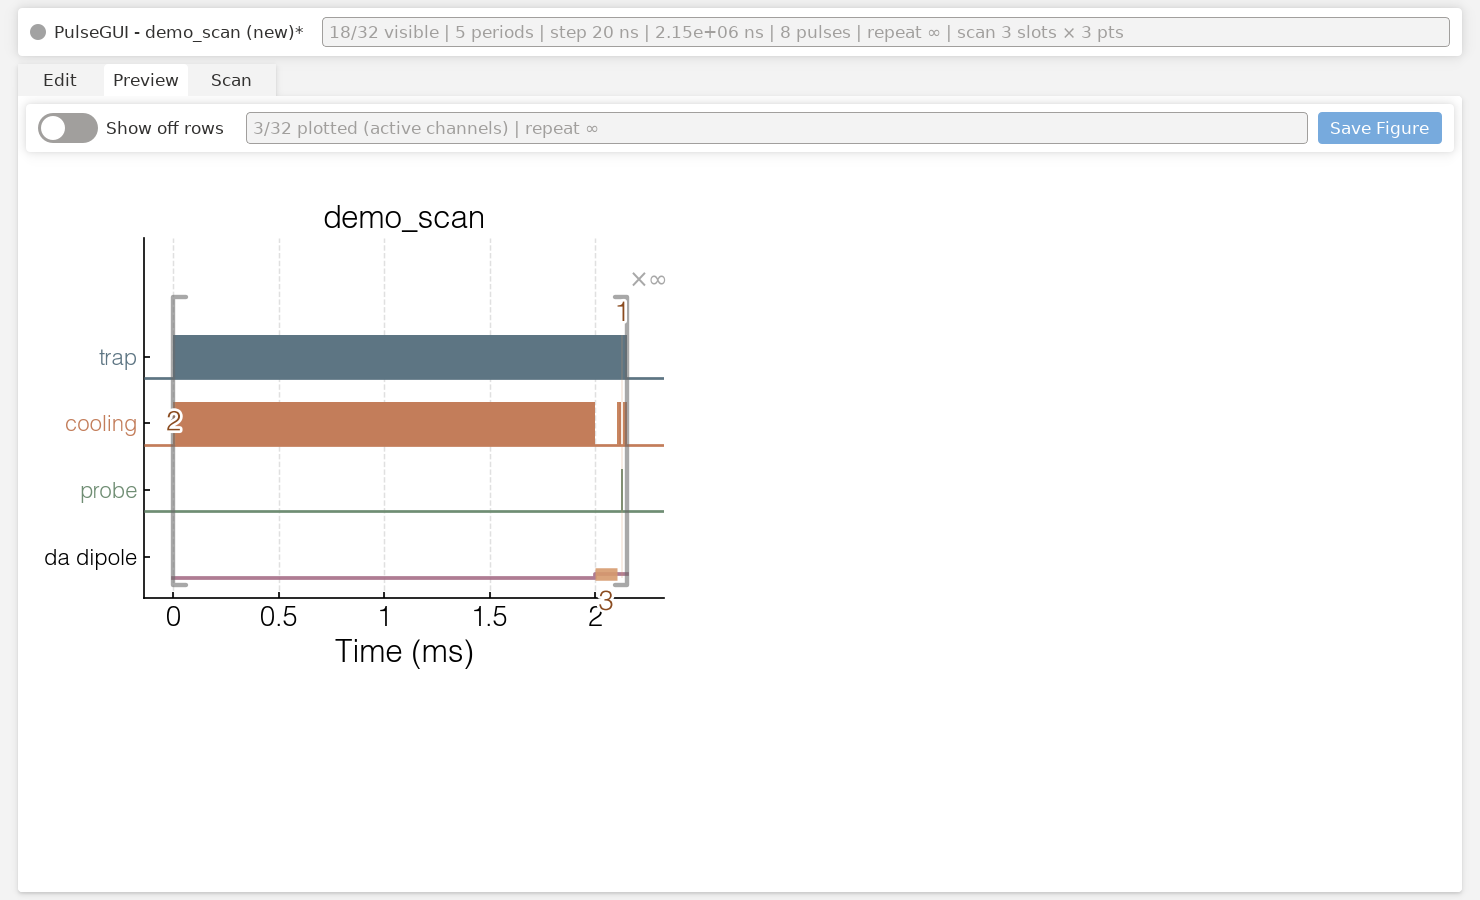
\includegraphics[width=\textwidth]{assets/frontend_gui_preview.png}
  \caption{Preview 页整体外观：顶部是 "Show off rows" 开关、状态标签与 "Save Figure" 按钮，下方是脉冲时间图；图中橘色透明区域就是扫描高亮，每个高亮带着它的 1 基槽位编号。}
\end{figure}

\subsection{它什么时候重画：没有"刷新"按钮}

在你动手找按钮之前，先记住一件最重要的事：\tfocus{Preview 页是自动重画的，根本没有手动刷新按钮}。

\begin{description}
\item[自动重画的时机] 只要你\tfocus{切换到 Preview 这个标签页}，或者\tfocus{在本页里拨动任何一个开关}，整张图就会立刻重新生成一遍。你不需要、也找不到一个"刷新""重画""更新预览"之类的按钮——因为根本不存在。
\item[画的是哪一份数据] 它画的是\tfocus{未展开的周期表}，也就是\tfocus{只画一次循环（one iteration）}的样子。如果你的序列里有"重复 N 次"这种结构，预览\tfocus{不会}把它真的铺开成 N 份重复的波形，而是画一次、再用括号和倍数标注（详见后文的 repeat 小节）。这样图不会因为重复几百次而变得无法阅读。
\item[常见的坑] 新手最容易困惑的是："我在 Edit 页改了参数，回到 Preview 怎么还是旧的？"——只要你是\tfocus{切换标签页}过来的，它就已经按最新数据重画了。如果你怀疑没更新，最稳妥的办法是切走再切回 Preview，强制触发一次重画。
\item[实用提示] 边调参数边看效果时，养成"改完就切回 Preview 瞄一眼"的习惯。因为重画是免费且自动的，多看几次不会有任何代价，反而能在发脉冲前就抓出明显的错误（比如某个通道一直是空的、某个延迟把边沿推到了奇怪的位置）。
\end{description}

\subsection{"Show off rows" 开关：要不要画一直关着的通道}

这是页面顶部的一个开关（toggle），标签写着 \pyapi{Show off rows}（显示关闭的行）。

\begin{description}
\item[作用] 它决定预览图里\tfocus{要不要把那些自始至终都没亮过的通道也画出来}。
\item[接受什么值] 它是一个二选一的开关，只有两种状态：\tfocus{关（off）}和\tfocus{开（on）}。没有中间档，也不接受数字输入。
\item[关（off）时会发生什么] 这是默认、也是最常用的状态。图里\tfocus{只画那些至少高电平过一次的通道}——也就是"在这次循环里干过活"的行。一直保持低电平、从头到尾没亮过的通道会被\tfocus{隐藏}，图会显得干净、紧凑，你能把注意力放在真正有脉冲的通道上。
\item[开（on）时会发生什么] 一旦打开，图里\tfocus{连那些一直关着的通道也会画出来}。结果就是多出一大堆\tfocus{空荡荡的行}（这些行从头到尾没有任何填充的条），图会一下子变高、变长。它的用处是：当你想确认"某个我以为该用上的通道，是不是其实一直没被触发"时，打开它就能一眼看到那条空行确实在、且确实是空的。
\item[常见的坑] 打开后图里突然冒出几十行空白，新手会以为"出错了"或"通道全废了"。其实那只是把平时藏起来的常关通道显示出来而已，属于正常现象。看完记得拨回去，否则后续每次预览都拖着一堆空行，不好读。
\item[实用提示] 日常调试让它\tfocus{保持关}，图最清爽；只有在排查"为什么某通道没动静"时才临时打开。开→关来回切换是安全的，图会稳定地回到一致的状态，不会因为切换次数多了就乱掉。
\end{description}

\subsection{状态标签与 "Save Figure" 按钮}

在开关旁边还有两样东西：一个\tfocus{状态标签}和一个 \pyapi{Save Figure}（保存图像）按钮。

\begin{description}
\item[状态标签（作用）] 这是一行文字提示，用来告诉你当前预览的状态信息。它不接受输入、也不能点——纯粹是给你看的。当你不确定图是不是最新、或者保存动作有没有成功时，瞄一眼这里通常能得到线索。
\item[Save Figure 按钮（作用）] 点它可以把\tfocus{当前这张预览图原样保存成一个 .png 图片文件}。这样你就能把波形截图贴进实验记录、汇报或手册里，而不必自己去截屏。
\item[点下去会发生什么] 按下后，程序会把现在屏幕上看到的这张图导出为一个 \pyapi{.png} 文件。导出的内容就是当下的样子——包括你此刻的 "Show off rows" 状态和所有橘色扫描高亮，所见即所存。
\item[常见的坑] 因为存的是"当下这一刻"的图，所以\tfocus{保存前要先把图调成你想要的样子}：该开/关的行先设好，确认扫描高亮显示正确，再点保存。如果你保存完才发现某通道没显示出来，多半是 "Show off rows" 的状态不对，调好再存一次即可。
\item[实用提示] 给保存的文件起个能认出实验配置的名字（比如带上序列名或日期），方便日后翻找。配合本手册前面提到的"保存脉冲会一起产出 pulse.json + png + scan 数组"的流程，这里手动导出的 png 适合用来单独抓某一帧你特别想留档的预览。
\end{description}

\subsection{图本身：数字通道行与模拟（DAC）行怎么画}

图的主体是一格一格的行。理解这张图的关键是分清\tfocus{两类行}：数字通道行，和模拟（DAC 总线）行。

\begin{description}
\item[数字通道行（每个通道一行）] 每一个数字通道占\tfocus{一行}。在这条行上，凡是该通道处于\tfocus{高电平}的时间段，都会画成一条\tfocus{填充的实心条（bar）}；低电平的时间段则是空白。所以你横着看一行，就能读出这个通道在一次循环里"什么时候开、什么时候关、开多久"。
\item[模拟（DAC）总线行（一条总线一行）] 每一条模拟 DAC 总线只占\tfocus{一行}，而且画法和数字行不同：它画的是\tfocus{一条阶梯线（step line）}，这条线的高度\tfocus{跟随该总线的真实数值}上下走。数值为 \pyapi{0} 时，线\tfocus{贴在基线上}；数值越大，线抬得越高。请特别注意：\tfocus{每条模拟行只有一条线，不是两条}——不要去找"上下两条边界线"，就是一条随值起伏的台阶线。
\item[总线的比特通道去哪了] 一条 DAC 总线在底层是由很多比特（bit）通道拼出来的。在预览里，这些\tfocus{比特通道总是被折叠进那一条模拟行}，\tfocus{绝不会}被单独拆成一行一行的数字通道显示。换句话说，你在数字行区域\tfocus{看不到} DAC 的某个 bit；它们全部归并到那条阶梯线里。
\item[常见的坑] 新手常犯两个错：一是想在数字行里找 DAC 的某根 bit，结果找不到——那是设计如此，bit 永远折叠进模拟行；二是看到阶梯线贴着底就以为"这行没在工作"，其实贴底只代表当前值是 0，线还是在的。
\item[实用提示] 读模拟行时，把注意力放在\tfocus{台阶的高度变化}上：每一级台阶就是一次新的 DAC 取值。想确认某段时间 DAC 是不是输出了你设定的码值，顺着那条线找对应时间点的高度即可。
\end{description}

\subsection{repeat（重复）：×∞、×N 与那个大括号}

预览只画一次循环，但它会用\tfocus{标注}告诉你这段序列实际会重复多少次。

\begin{description}
\item[无限循环：×∞ 加一个大括号] 如果整段序列是\tfocus{无限重复}的，图上会显示 \pyapi{×∞}，并配一个\tfocus{横跨整段序列的大括号（bracket）}，把这段会被反复执行的区域整个圈起来。这个括号是在告诉你："括号里的内容会一遍又一遍地跑下去。"
\item[有限内层循环：×N] 如果某一段是\tfocus{有限次}的内层循环，它会标成 \pyapi{×N}（N 是具体的重复次数），同样用括号圈出它覆盖的范围。于是你能同时看到"外层无限 ×∞"和"内层若干次 ×N"两层标记并存。
\item[永远不会出现 "inf" 这个词] 请注意，图里\tfocus{从不出现字面的英文 "inf"}。无限重复\tfocus{只}用 \pyapi{×∞} 这个符号表示。如果你在哪儿看到了 "inf"，那不是这套预览该有的输出。
\item[延迟把边沿推到表尾之外时会怎样] 这是一个容易吓到新手的细节：通道延迟（delay）可能把某个边沿\tfocus{推到周期表末尾之后}。这种情况下，\tfocus{×∞ 的大括号会自动延伸，把这个被推出去的边沿也包进来}，\tfocus{绝不会有任何东西画在循环括号之外}。直观地说就是"括号会自己变长去兜住那条迟到的边沿"，让整张图读起来始终是物理上自洽的——一切都在循环之内。
\item[常见的坑] 如果你没意识到延迟会延长括号，可能会困惑"为什么这个 ×∞ 括号比序列正文还长一点"。那正是延迟造成的，是正确行为，不是 bug。
\item[实用提示] 看 repeat 标记时，先找最外层的 ×∞ 确认整体是不是无限跑，再逐个看内层的 ×N 核对每段重复次数对不对。如果发现括号右端伸得比你预期长，去检查相关通道的延迟设置，多半就是它把边沿推出去了。
\end{description}

\subsection{扫描高亮（橘色透明）：三种被扫描的量怎么标}

这是 Preview 页最有特色的部分。当你把某个参数绑定为\tfocus{扫描槽位（scan slot）}时，预览会用\tfocus{透明的橘色}把这个参数在图上对应的位置高亮出来，并\tfocus{在该高亮上标一次它的槽位编号}。编号是 \tfocus{1 基（1-based）}的——也就是从 1 开始数，而不是从 0；每个高亮只标\tfocus{一次}编号，不会在同一段上重复盖好几个相同的数字。

下面分三种被扫描的量来讲，它们的高亮形状和编号位置各不相同，认清形状就能一眼分辨你扫的到底是哪一类量。

\begin{description}
\item[被扫描的 DURATION（周期时长）] 当你扫描某个周期的\tfocus{时长}时，高亮是一条\tfocus{橘色的竖向带子}，盖住\tfocus{这个周期所占的那段时间}。关键点：这条带子在纵向上\tfocus{只覆盖通道行的区域}——它的\tfocus{顶部恰好到最上面那条通道的顶}，\tfocus{绝不会再往上越过去}盖到标题那一带。它的\tfocus{槽位编号}写在\tfocus{最顶上通道正上方那一小条空隙（headroom）里}，刚好夹在通道和标题之间，\tfocus{不会和标题文字叠在一起}。这样你既能看清是哪个周期被扫，又不会让数字糊进标题。
\item[被扫描的 DELAY（通道延迟）] 当你扫描某个通道的\tfocus{延迟}时，高亮是一条橘色带子，盖在\tfocus{这个通道自己脉冲的"前导段（lead-in）"}上，而且\tfocus{就画在这条通道自己的行上}——它会\tfocus{精确落到正确的那条通道行}，不会跑到别的通道去。\tfocus{槽位编号}也写在\tfocus{这条通道的行上}。所以当你看到某条通道行的脉冲前面有一段橘色，就知道这条通道的延迟正被扫描。
\item[被扫描的 DAC 值] 当你扫描某条 DAC 总线的\tfocus{输出值}时，高亮\tfocus{跟着那条模拟阶梯线走}：它是一段\tfocus{位于该数值高度上的、短短的橘色线段}，只覆盖被扫描的那个周期，\tfocus{而不是把整行涂成一个色块}。也就是说，橘色出现在"线当前的高度"上，随值高低而高低。它的\tfocus{槽位编号}写在\tfocus{这条模拟行的正下方一点点}的位置。
\end{description}

\begin{notebox}[怎么靠形状区分三种扫描]
快速心法：橘色\tfocus{满高地盖住整段时间、数字在顶部通道上方} = 在扫\tfocus{周期时长}；橘色\tfocus{只盖某条通道脉冲的开头、数字在那条通道行上} = 在扫这条通道的\tfocus{延迟}；橘色\tfocus{是一小段贴着阶梯线高度的短线、数字在模拟行下方} = 在扫\tfocus{DAC 值}。记住这三种形状，你不用点任何东西就能读出自己到底在扫什么。
\end{notebox}

\begin{notebox}[编号为什么只出现一次]
即使一个被扫描的量在一次循环里跨了好几段（比如某通道在多个周期里都亮），它的槽位编号也\tfocus{只标在第一段上}，其余各段\tfocus{只上橘色、不再重复写数字}。这是有意为之，目的是避免同一个编号在一条通道上盖出好几个重叠的数字、把图弄花。所以\tfocus{一个槽位在图上恰好对应一个数字}——看到几个不同的数字，就代表你正在同时扫几个不同的槽位。
\end{notebox}

\section{Scan 页与扫描工作流（逐元素详解 + 实操配方）}

Scan 页是你\tfocus{搭建扫描表}（也就是扫描点列表）的地方。所谓"扫描表"，本质上是一张二维数表：每一\tfocus{行}代表实验要采集的一个\tfocus{扫描点}，每一\tfocus{列}代表一个被绑定的扫描槽（slot，记作 \pyapi{s0}、\pyapi{s1}、\pyapi{s2} ……）。当你在硬件上 On Pulse 时，序列器会从上到下逐行执行这张表，每一行对应硬件上的一次无缝扫描点，并且\tfocus{每个扫描点恰好发一次相机触发}。换句话说，扫描表有多少行，这一轮就采集多少个数据点。

在动手之前，先记住贯穿整页的核心约束：扫描表里你能引用的变量只有 \pyapi{s0} 到 \pyapi{s\{n-1\}}，没有历史遗留的 \pyapi{x}/\pyapi{y} 概念。每一列对应哪个物理量，是你在 Edit 页给某个字段点"扫描圆点"绑定时决定的——绑定第一个字段得到 \pyapi{s0}，第二个得到 \pyapi{s1}，以此类推。Scan 页本身不创建槽，它只负责给这些已存在的槽\tfocus{填数值}。

\begin{figure}[htbp]
  \centering
  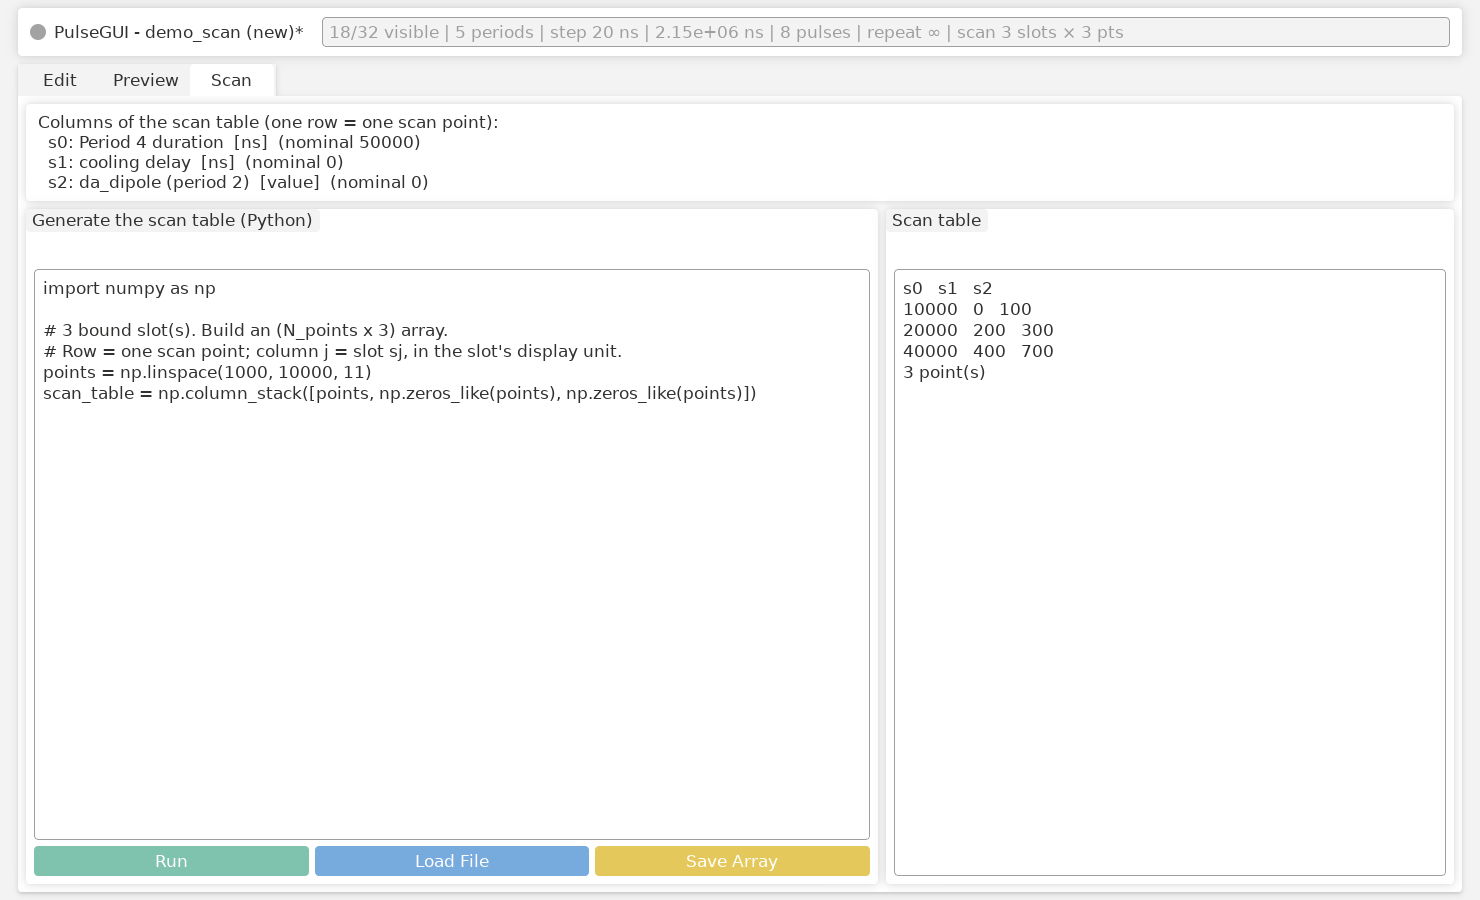
\includegraphics[width=\textwidth]{assets/frontend_gui_scan.png}
  \caption{Scan 页整体布局：顶部是各列含义说明，中间是白色 Python 代码编辑器，下方是 Run / Load File / Save Array 按钮和只读的扫描表预览。}
\end{figure}

\subsection{顶部：扫描表列含义说明（Columns of the scan table）}

页面最顶部是一块\tfocus{只读的说明文字}，每一个被绑定的扫描槽占一行，告诉你这张表的每一列到底代表什么物理量、属于哪个周期或通道、以及它的\tfocus{单位}。

\begin{description}
\item[它显示什么] 每行形如 \pyapi{s0: Period 4 duration [ns] (nominal 50000)}、\pyapi{s1: cooling delay [ns]}、\pyapi{s2: da\_dipole (period 2) [value]}。冒号前是槽号（与代码里要用的变量名一一对应），冒号后是这个槽绑定到的字段的人类可读描述：是哪个周期的 duration、哪个通道的 delay、还是哪个周期的某个 DAC 总线值。
\item[单位约定] 方括号里的单位非常关键。时间类的槽（duration、delay）单位是 \pyapi{[ns]}（纳秒），你在代码里填的数字就按纳秒理解；DAC 类的槽单位是 \pyapi{[value]}，表示\tfocus{原始 DAC 码}（raw code），不是电压、也不是纳秒，取值范围是整数 \pyapi{0} 到 \pyapi{1023}。把这两类单位搞混是新手最常见的错误。
\item[nominal 标注] 对于像 duration 这样有标称值的槽，括号里会附带 \pyapi{(nominal 50000)}，告诉你这个字段在 Edit 页填的原始值是多少。它是一个\tfocus{参照基准}：你可以围绕这个标称值设计扫描范围（比如以 50000 ns 为中心上下扫），心里好有个数。
\item[点击后会发生什么] 这块区域是纯展示，\tfocus{不能点击、不能编辑}。它会随着你在 Edit 页绑定/解绑字段而自动刷新行数和内容——你在 Edit 多绑一个字段，这里就多出一行 \pyapi{s\{下一个号\}}。
\item[常见坑] 如果这里\tfocus{一行都没有}（显示类似"无扫描槽"的占位提示），说明你还没在 Edit 页绑定任何字段，此时写再多代码也没有列可填。请先回 Edit 页点亮至少一个扫描圆点。
\item[实用提示] 写代码前，先照着这块说明从上往下数一遍：第 0 行就是 \pyapi{scan\_table} 的第 0 列，第 1 行就是第 1 列……让脑子里的"列序"和说明里的"槽序"对齐，能避免把 duration 的数填进 DAC 列这类张冠李戴的错误。
\end{description}

\subsection{中间：Python 代码编辑器}

中间一大块\tfocus{白底等宽字体}的区域是 Python 代码编辑器。你在这里写一小段 Python 代码，\tfocus{把一个形状为 N\_points × N\_slots 的数组赋值给变量 }\pyapi{scan\_table}。点 Run 时，这段代码会被执行，结果写回状态并刷新下方预览。

\begin{description}
\item[作用] 它是构建扫描表最灵活的方式：用代码生成任意规则或不规则的扫描点序列（等间距、对数、随机、网格……），远比手动敲数字高效。
\item[可用的命名空间] 代码执行时，环境里已经为你准备好了：\pyapi{numpy}（以 \pyapi{np} 名字提供）、\pyapi{math} 模块，以及整数 \pyapi{n\_slots}（当前被绑定的槽数量，等于扫描表应有的列数）。你可以直接用 \pyapi{np.linspace}、\pyapi{np.arange}、\pyapi{np.column\_stack} 等，无需自己 import。
\item[必须满足的契约] 代码运行完，命名空间里\tfocus{必须存在}一个名为 \pyapi{scan\_table} 的变量，且它是一个二维数组：行数 = 扫描点个数（你自己定，比如 21、50、100），列数 = \pyapi{n\_slots}。第 \pyapi{j} 列填的就是槽 \pyapi{s\{j\}} 在它\tfocus{显示单位}下的数值（时间槽填 ns、DAC 槽填 0..1023 的码）。
\item[点击 Run 后会发生什么] 见下一小节。简单说：代码被执行，\pyapi{scan\_table} 被读出并写回状态，下方预览随即刷新。
\item[常见坑] （1）忘了把结果命名成 \pyapi{scan\_table}，或者拼错变量名；（2）数组列数和 \pyapi{n\_slots} 不一致——比如绑了 3 个槽却只给了 2 列；（3）把 DAC 列写成了纳秒级的大数（如 50000），而 DAC 码合法范围只有 0..1023；（4）写成一维数组而忘了它需要是二维（哪怕只有一个槽，也应是 N×1 的形状）。
\item[实用提示] 善用 \pyapi{n\_slots} 让代码自适应：用 \pyapi{np.column\_stack([...])} 按列拼装，每个槽一列，顺序严格对应顶部说明里的 \pyapi{s0, s1, ...}。先在脑中确认"第几列是哪个物理量"，再动手拼列，能一次写对。
\end{description}

\subsection{Run 按钮（绿色）}

\begin{description}
\item[作用] 绿色的 Run 按钮\tfocus{执行}上方代码编辑器里的 Python 代码。
\item[点击后会发生什么] 代码被运行，运行结束后系统从命名空间里取出 \pyapi{scan\_table} 变量，把它\tfocus{写回实验状态}，然后刷新下方那张只读的扫描表预览，让你立刻看到生成结果。
\item[接受什么] 它不接受参数，就是一个执行触发器；真正的"输入"是你在编辑器里写的代码。
\item[常见坑] 如果代码有语法错误、引用了未定义的名字、或最终没有产出合法的 \pyapi{scan\_table}，Run 就无法把有效结果写回。每次改完代码都要重新点 Run，否则状态里还是上一次的旧表——\tfocus{只编辑不 Run 等于没生效}。
\item[实用提示] 把 Run 当成"编译并预览"这一步：改代码 → Run → 看下方预览的行数和前几行数值是否符合预期，确认无误再去 On Pulse。养成这个习惯能避免拿着错误的扫描表上硬件。
\end{description}

\subsection{Load File 按钮}

\begin{description}
\item[作用] Load File 让你\tfocus{从文件载入}一张现成的扫描表，作为写代码之外的另一条路径。
\item[接受什么] 支持 \pyapi{.npy}、\pyapi{.csv}、\pyapi{.txt} 三种格式的数组文件。文件里应是一张二维数表，行 = 扫描点、列 = 槽，列序同样要对应顶部说明的 \pyapi{s0, s1, ...}。
\item[点击后会发生什么] 弹出文件选择框，选中文件后表内容被读入并写回状态，下方预览刷新显示载入的内容。这相当于跳过代码编辑器，直接把外部生成（比如别的脚本、Excel 导出）的扫描点拿来用。
\item[常见坑] 文件的\tfocus{列数必须等于当前绑定的槽数}，单位也要对（时间列是 ns、DAC 列是 0..1023 的整数码）；列顺序如果和顶部说明对不上，物理量就会错位。从 \pyapi{.csv}/\pyapi{.txt} 载入时还要留意分隔符和是否带表头行。
\item[实用提示] 如果你的扫描点来自标定脚本或事先算好的网格，用文件载入比把整段生成逻辑塞进代码框更清爽；可以先用 Save Array 存一份标准 \pyapi{.npy}，之后反复 Load File 复用。
\end{description}

\subsection{Save Array 按钮}

\begin{description}
\item[作用] Save Array 把\tfocus{当前的扫描表}保存成一个数组文件，方便归档、复用或在别处分析。
\item[点击后会发生什么] 弹出保存对话框，把现在状态里的扫描表（也就是你刚 Run 出来或 Load 进来的那张）写到磁盘。
\item[接受什么] 你指定保存路径与文件名；保存出来的就是和扫描表同形状的二维数组文件。
\item[常见坑] 它保存的是\tfocus{当前状态里的表}，所以保存前请确认你已经 Run 过、预览里显示的就是你想要的内容；否则可能把一张旧表或空表存下来。
\item[实用提示] 给文件起带含义的名字（比如包含被扫物理量和范围），并和对应的 pulse 配置存在一起，日后回溯"这组数据是怎么扫的"会轻松很多。
\end{description}

\subsection{下方：只读扫描表预览}

\begin{description}
\item[作用] 编辑器下方是一张\tfocus{只读}的扫描表预览，按 \pyapi{s0}/\pyapi{s1}/\pyapi{...} 列展示扫描表的\tfocus{前若干行}，并显示总的扫描点数（point count）。
\item[它告诉你什么] 这是你"所写即所得"的核对窗口：列名让你确认每一列对应哪个槽，前几行数值让你检查范围和步长是否正确，点数让你确认这一轮会采多少个点（也就是会发多少次相机触发）。
\item[点击后会发生什么] 它\tfocus{不可编辑}，纯展示。每次 Run 或 Load File 后它会自动刷新。
\item[常见坑] 它通常只显示前几行，别因为没看到全部行就以为表被截断了——以显示的\tfocus{总点数}为准。如果点数或列数和你预期不符，回到代码或文件去查，而不是试图在预览里改。
\item[实用提示] 上硬件前，最后扫一眼这里的\tfocus{点数}和\tfocus{第一行/最后一行}（如果能看到），快速验证扫描范围的两个端点是否如你设计，这是最省事的"出错前一刻"检查。
\end{description}

\subsection{完整工作流：四步走}

把整个扫描串起来，一共四步，前面在 Edit 页，后面在 Scan 页和运行：

\begin{enumerate}
\item \tfocus{在 Edit 页绑定字段}：找到你想扫的字段（某周期的 duration、某通道的 delay、或某周期的 DAC 总线值），点它旁边的\tfocus{扫描圆点}。第一个绑定的字段成为 \pyapi{s0}，第二个成为 \pyapi{s1}，依次类推。绑定后该字段会被高亮标记并显示槽号。
\item \tfocus{在 Scan 页写代码}：照着顶部"列含义说明"确认每一列是哪个槽、什么单位，然后在代码编辑器里构造一个 N\_points × \pyapi{n\_slots} 的数组并赋给 \pyapi{scan\_table}。
\item \tfocus{点 Run}：执行代码，把 \pyapi{scan\_table} 写回状态，并在下方预览核对行数、列、数值。
\item \tfocus{On Pulse 运行}：硬件\tfocus{无缝}地逐行执行这张扫描表，每个扫描点对应一次相机触发。一轮跑完，你就得到了对应所有扫描点的数据。
\end{enumerate}

\begin{notebox}[一句话记忆]
Edit 页\tfocus{绑定}决定有几列（\pyapi{s0, s1, ...}），Scan 页\tfocus{填数}决定有几行（扫描点）。列错了回 Edit，行错了回代码。
\end{notebox}

\subsection{实操配方一：一维 duration 扫描}

最常见的需求：固定其它一切，只扫某个周期的持续时间。假设你在 Edit 页只绑定了一个字段（某周期的 duration），它是 \pyapi{s0}，单位 ns，标称值 \pyapi{50000}。下面这段代码以标称值为中心、从 \pyapi{40000} ns 到 \pyapi{60000} ns 扫 \pyapi{21} 个等间距点：

\begin{codeblock}[Python]
# 只绑定了一个 duration 槽 s0（单位 ns）
durations = np.linspace(40000, 60000, 21)   # 21 个点，含两端
scan_table = durations.reshape(-1, 1)        # 形状 (21, 1) = N_points x n_slots
\end{codeblock}

\begin{description}
\item[要点] \pyapi{linspace(a, b, n)} 生成含两端、共 \pyapi{n} 个等间距值；\pyapi{reshape(-1, 1)} 把一维数组变成 N×1 的二维表（一列对应唯一的槽 \pyapi{s0}）。
\item[常见坑] 别忘了 \pyapi{reshape}——一维数组不满足"二维 N×slots"的契约；时间值用 ns，别误填成别的单位。
\item[提示] 想换成对数扫描就把 \pyapi{np.linspace} 换成 \pyapi{np.logspace}；想改点数只改第三个参数，预览里的 point count 会立刻反映出来。
\end{description}

\subsection{实操配方二：扫一个 DAC 电平（原始码 0..1023）}

如果你绑定的是一个 DAC 总线值字段（\pyapi{[value]} 单位），它对应原始 DAC 码，合法范围是整数 \pyapi{0} 到 \pyapi{1023}。假设它是唯一绑定的槽 \pyapi{s0}，下面在整个量程上扫 \pyapi{32} 个点：

\begin{codeblock}[Python]
# 只绑定了一个 DAC 值槽 s0（原始码 0..1023）
codes = np.linspace(0, 1023, 32).round().astype(int)
scan_table = codes.reshape(-1, 1)            # 形状 (32, 1)
\end{codeblock}

\begin{description}
\item[要点] DAC 列填的是\tfocus{整数原始码}，所以用 \pyapi{round().astype(int)} 取整；范围务必落在 \pyapi{0}..\pyapi{1023} 之内。
\item[常见坑] 把 DAC 列当成电压或纳秒来填（写出 50000 这种数）会超出 \pyapi{1023} 的合法范围；浮点码也不合适，记得取整。
\item[提示] 只想扫量程的一部分（比如偏置点附近），把 \pyapi{linspace} 的两端改成你关心的码区间即可。
\end{description}

\subsection{实操配方三：二维扫描（duration × DAC）}

二维扫描就是把两个槽的取值做\tfocus{笛卡尔网格}，每个组合是一个扫描点。假设 \pyapi{s0} 是 duration（ns），\pyapi{s1} 是 DAC 码（0..1023）。下面构造一个 \pyapi{11 × 8 = 88} 点的网格：

\begin{codeblock}[Python]
# s0 = duration [ns], s1 = DAC value [0..1023]
durs  = np.linspace(40000, 60000, 11)        # 11 个 duration
codes = np.linspace(0, 1023, 8).round().astype(int)  # 8 个 DAC 码

# 笛卡尔积：每个 (duration, code) 组合一行
D, C = np.meshgrid(durs, codes, indexing="ij")
scan_table = np.column_stack([D.ravel(), C.ravel()])  # 形状 (88, 2)
\end{codeblock}

\begin{description}
\item[要点] \pyapi{np.meshgrid(..., indexing="ij")} 配 \pyapi{ravel()} 展平，再用 \pyapi{np.column\_stack} 按\tfocus{槽序}拼成两列——第 0 列是 \pyapi{s0}（duration），第 1 列是 \pyapi{s1}（DAC）。列序必须和顶部说明一致。
\item[常见坑] 列放反（把 DAC 码放进 duration 列）会让两个物理量错位；网格点数是两边相乘，点数容易爆炸，先在预览里确认 point count 别太大。
\item[提示] 想加第三维（比如再扫一个 delay 槽 \pyapi{s2}），把它也放进 \pyapi{meshgrid} 并在 \pyapi{column\_stack} 里加一列即可。
\end{description}

\begin{notebox}[同时扫多个物理量]
DAC 值、duration、delay 三类槽\tfocus{可以在同一轮里一起扫}。你在 Edit 页绑定几个字段、Scan 页就给几列填数，硬件会按行无缝执行这张多列扫描表，每个扫描点照常发一次相机触发。这让"沿某条轨迹同步改变多个参数"或"多维网格扫描"成为一次 On Pulse 就能完成的事。
\end{notebox}

\chapter{完整走一遍（新手教程）}
本章假设你\tfocus{从零开始}，一步步搭一个真实的脉冲序列、预览、再加一个扫描。每一步对应上一章讲过的控件，配合 Edit/Preview/Scan 三张截图看。

\section{第 0 步：打开编辑器}
从命令行：

\begin{codeblock}[PowerShell]
.\pulse_gui.bat
\end{codeblock}

或在 notebook 里：

\begin{codeblock}[Python]
from Zou_lab_control.frontend.pulse_gui import PulseSequenceEditor
from Zou_lab_control.frontend.qt_fluent import ensure_qt_app
app = ensure_qt_app()
ed = PulseSequenceEditor()        # 空白脉冲表
ed.show(); app.exec_()
\end{codeblock}

打开后默认停在 \tfocus{Edit} 页。顶部三个标签 \pyapi{Edit / Preview / Scan}，顶部状态条显示可见数、period 数、step、总时长等。

\section{第 1 步：理解“一段就是一张卡片”}
脉冲序列不是网格表，而是一排\tfocus{周期卡片（period）}，每张卡是一段持续时间。中间区域横向排着 \pyapi{Period 1/5}、\pyapi{Period 2/5}……每张卡上有这一段的时长、单位、和每条 channel 的勾选框。时间从左到右流动。

\section{第 2 步：加 / 删一段，设时长}
\begin{enumerate}
  \item 点底部 \pyapi{Add Period} 增加一段（点 \pyapi{Remove} 删除当前段）。
  \item 在某张卡的 \pyapi{Duration} 框里填时长，右边下拉选单位（\pyapi{ns/us/ms/s}）。例如第一段填 \pyapi{2 ms}（磁光阱加载），第二段填 \pyapi{100 us}。
\end{enumerate}

\section{第 3 步：让 channel 在某些段为高}
在每张卡上，勾选要在这段时间内\tfocus{打开}的 channel（勾上=高电平）。例如让 \pyapi{trap} 在所有段都勾上、\pyapi{cooling} 只在加载段勾上、\pyapi{probe} 只在成像段勾上。左侧 \pyapi{Channel Names} 列可以给每条 channel 起个好记的名字。

\section{第 4 步：设延时（可选）}
在 \pyapi{Delay / Scan} 列，给某条 channel 的延时框填一个值（可正可负），用来补偿器件/线缆时延。延时只平移这条 channel 的开关沿，不改变周期长度。

\section{第 5 步：在 Preview 看波形}
点 \pyapi{Preview} 标签。它画出\tfocus{未展开}的周期表：每条数字 channel 一行方波，模拟总线一行阶梯线。切 \pyapi{Show off rows} 开关可显示/隐藏全程为 0 的 channel。这一页只看、不改；改完 Edit 再回来会自动重画。

\section{第 6 步：把一个字段变成扫描参数}
回到 Edit 页，决定要扫什么：
\begin{enumerate}
  \item 点某个 duration / delay / DAC 值框右边的\tfocus{扫描圆点}（图~\ref{fig:fe-dot}）。该字段变淡橙、显示它的 slot 编号（第一个绑定的是 1）。
  \item 想扫第二个参数就再点另一个字段的圆点（编号 2），以此类推。
\end{enumerate}

\section{第 7 步：在 Scan 页填扫描表}
点 \pyapi{Scan} 标签。顶部列出每个 slot 是哪个字段、什么单位。在 Python 代码框里构造一个 \pyapi{N_points x N_slots} 的数组赋给 \pyapi{scan_table}，点 \pyapi{Run}：

\begin{codeblock}[Scan 页：扫一个 duration]
import numpy as np
# 单 slot：把绑定的那个时长从 1 us 扫到 10 us，共 10 个点。
scan_table = np.linspace(1000, 10000, 10).reshape(-1, 1)   # 单位 ns
\end{codeblock}

也可以点 \pyapi{Load File} 从 \filepath{.npy}/\filepath{.csv}/\filepath{.txt} 直接载入，或 \pyapi{Save Array} 把表存出来。

\section{第 8 步：运行 / 保存}
\begin{enumerate}
  \item 回 Edit 页，点 \pyapi{On Pulse}：它先把当前脉冲编译上传到 sequencer，再启动。硬件会无缝地逐个扫描点跑，每点触发一次相机。
  \item \pyapi{Stop Pulse} 让输出回到安全态。
  \item \pyapi{Save} 把脉冲 \filepath{.json} + 预览 \filepath{.png} +（有扫描表时）扫描数组一起存出，三件配套。
\end{enumerate}

\section{完整例子：扫一个 DAC（DA）电平}
把上面串起来，做实验里最常用的“扫 DA”：
\begin{enumerate}
  \item Edit 页搭好脉冲；在某一段把某条模拟总线（如 \pyapi{da_dipole}）的 DAC 值框的扫描圆点点亮。
  \item Scan 页填\tfocus{原始 10-bit DAC 码}（0..1023，不是电压、不是 ns）：
\end{enumerate}

\begin{codeblock}[Scan 页：扫 DAC 码]
import numpy as np
scan_table = np.linspace(0, 1000, 11).astype(int).reshape(-1, 1)
\end{codeblock}

\begin{enumerate}
  \setcounter{enumi}{2}
  \item \pyapi{Run} 写回，回 Edit 页 \pyapi{On Pulse}。FPGA 逐点切 DAC，硬件无缝（无需每点重传）。在 Preview 里，被扫的 DAC 段会高亮显示在\tfocus{它那条总线的行上}并标着 slot 编号。
\end{enumerate}

\section{遇到问题先看哪里}
\begin{description}
  \item[Preview 不出图] 切一下 \pyapi{Show off rows} 触发重画；确认脉冲表非空、最后一段把所有 channel 归零。
  \item[扫描报错] 确认每个扫描点是 20 ns 的整数倍（时间 slot）；DAC 用原始码；duration 扫描不要和 DAC 扫描混用。
  \item[On Pulse 无信号] 见主手册“真实硬件 Runbook / 常见问题”。
\end{description}

\chapter{绘图 API}

\section{统一的数组契约}
\pyapi{Zou_lab_control.frontend.plot} / \pyapi{live} 用同一套数组契约：\pyapi{data_x} 是 \pyapi{(N, coord_dim)}，\pyapi{data_y} 是 \pyapi{(N, channel_dim)}。\pyapi{coord_dim == 1} 画一维线图，\pyapi{coord_dim == 2} 画二维扫描图，\pyapi{kind="hist"} 把 \pyapi{data_x} 当作数值数组。未完成的数据用 \pyapi{NaN} 表示，前端可据此推断进度。

\begin{codeblock}[Python]
import numpy as np
from Zou_lab_control.frontend import plot

x = np.linspace(737.0, 737.2, 220).reshape(-1, 1)
y = (lorentzian(x) + noise).reshape(-1, 1)
p = plot(x, y, labels=("Wavelength (nm)", "Counts/0.1s", "Counts"))
p.data_figure.lorent(is_display=True)      # 叠加洛伦兹拟合
\end{codeblock}

\begin{figure}[htbp]
  \centering
  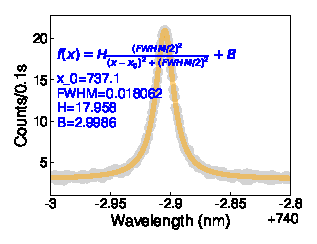
\includegraphics[width=0.82\textwidth]{assets/frontend_1d_fit.pdf}
  \caption{一维线图加洛伦兹拟合。}
\end{figure}

\begin{figure}[htbp]
  \centering
  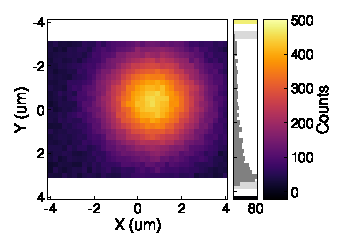
\includegraphics[width=0.78\textwidth]{assets/frontend_2d_scan.pdf}
  \caption{二维扫描图：data\_x 为 (N, 2)，data\_y 为 (N, 1)。}
\end{figure}

\section{直方图与阈值}
\begin{codeblock}[Python]
hist = plot(roi_counts, kind="hist", bins=55, thresholds=[45],
            labels=("ROI counts", "Shots", "Population"))
\end{codeblock}

\begin{figure}[htbp]
  \centering
  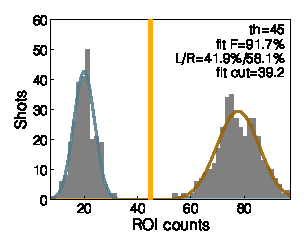
\includegraphics[width=0.78\textwidth]{assets/frontend_histogram.pdf}
  \caption{带阈值的 ROI 计数直方图，用于亮/暗判定。}
\end{figure}

\section{实时刷新}
用 \pyapi{update="watch"} 时，返回对象启动一个前端定时器，从共享数组刷新，而采集代码在另一侧 in-place 修改这些数组。worker 不直接动 Matplotlib artist；前端拥有 artist 和刷新。绘图刷新依赖事件循环，因此阻塞式硬件采集不能直接跑在 UI 线程里。

\chapter{PDF 渲染 API}

\section{render\_tex\_pdf}
一次性从 TeX 串或 \filepath{.tex} 文件生成 PDF，首选 \pyapi{render_tex_pdf}。它在临时目录里编译（XeLaTeX 两遍），只把最终 PDF 拷回，调用方不必管 \filepath{.aux}/\filepath{.log} 等辅助文件。

\begin{codeblock}[Python]
from Zou_lab_control.frontend.notes import render_tex_pdf

render_tex_pdf("docs/main_manual/main_manual_zh.tex",
               "docs/main_manual/main_manual_zh.pdf")
\end{codeblock}

输入是 \filepath{.tex} 文件时，同目录的资产（如 \filepath{assets/foo.pdf}）会被拷进临时构建树，但同名的旧输出（\filepath{.pdf}/\filepath{.aux}/\filepath{.log}/\filepath{.build.log}）不会被拷。构建失败时只在输出 PDF 旁留一个 \filepath{.build.log} 供诊断（包括 XeLaTeX 缺失或路径错误的情况）。

\section{notes 风格的整本手册}
\pyapi{render_notes_pdf(..., clean_compile=True)} 用同一个干净编译器，自动套用本仓库的标题页与目录样式。\pyapi{render_latex_pdf_clean(...)} 是兼容别名。本手册自身就是用这条路径生成的（见 \filepath{Zou_lab_control/frontend/notes.py} 里的 \pyapi{build_frontend_manual}）。

\chapter{修改指南}

\section{我要加一个新 Fluent 控件}
扩展 \filepath{qt_fluent.py}，复用 \pyapi{Metrics} token 和 \pyapi{scaled_px()}，不要在 GUI 模块里另造样式或缩放。新控件应能在 \pyapi{FluentFormGrid} 里以 \pyapi{Metrics.row_h()} 高度对齐。

\section{我要给脉冲 GUI 加一行}
任何新行、spacer、标题、开关文字或局部 margin，都必须保证 \pyapi{Channel Names}、\pyapi{Delay \& Scan}、period 卡片、repeat bracket 这几块的顶部控制行仍然对齐。改完后加 object-level 断言：同一 channel 的 raw 标签、延时框、第一个 period 勾选框的 y 坐标相等。

\section{我要改截图 QA}
截图前必须跑事件循环并等待；\pyapi{show()} 或状态变化后不要立刻 \pyapi{grab()}：

\begin{codeblock}[Python]
editor.show()
editor.grab_screenshot(path, settle_ms=1000)        # 首选 helper
# 没有 helper 时:
# app.processEvents(); QtTest.QTest.qWait(1000); app.processEvents(); editor.grab().save(path)
\end{codeblock}

离屏截图可能漏字，所以截图只作视觉 QA；按钮文字、几何、状态仍要用 object-level 测试断言。更多规则见 \filepath{docs/MAINTAINER_NOTES.md}。

\section{我要改本手册}
正文模板在 \filepath{Zou_lab_control/frontend/content/manual_templates/frontend_manual_zh.texbody}，示例图由 \filepath{Zou_lab_control/frontend/content/manuals.py} 的 \pyapi{generate_frontend_manual_figures} 生成。改完用 \pyapi{build_frontend_manual()} 重建 PDF。


\end{document}
